
\newcommand{\nomedoc}{Piano Di Qualifica}
\newcommand{\versione}{5.0}
\newcommand{\versioneglossario}{4.0}
\newcommand{\versionenormeprogetto}{4.0}
\newcommand{\versioneAR}{3.0}
\newcommand{\versioneST}{3.0}
\newcommand{\nomefile}{PianoDiQualifica-\versione.pdf}
\newcommand{\datacreazione}{3 Dicembre 2010}
\newcommand{\datamodifica}{28 Marzo 2011}
\newcommand{\stato}{formale}
\newcommand{\uso}{esterno}
\newcommand{\redazione}{Trezzi Giovanni}
\newcommand{\verifica}{Palazzin Alberto}
\newcommand{\approvazione}{Lovato Daniele}
\newcommand{\distribuzione}{ 
VT.G \\
& Prof. Vardanega Tullio\\
& Prof. Cardin Riccardo }

% FUNZIONI TIPOGRAFICHE
\newcommand{\co}{\texttt} % courier
\newcommand{\bo}{\textbf} % bold
\newcommand{\pr}{\par\medskip} % paragrafo spaziato
\newcommand{\sca}{\textsc} % small caps

\documentclass[a4paper,12pt]{report}
% 10pt,11pt,12pt
% titlepage, notitlepage -> per dare inizio o no ad una nuova pagina dopo titolo
% twoside -> per dire se fronte-retro
\usepackage[latin1]{inputenc}
% per caratteri accentati
\usepackage[italian]{babel}
% per regole sintattiche italiane
\usepackage[bookmarks=true, pdfborder={0 0 0 0}]{hyperref}
% per collegamenti ipertestuali
\usepackage{graphicx}
% per inserimento immagini

% \usepackage{enumerate}
% per personalizzare elenchi puntati

\usepackage[hmargin=2cm]{geometry} %margine 2 cm
%\geometry{options varie}

% comandi per gestire meglio header e footer
\usepackage{fancyhdr}  % header e footer
\usepackage{totpages}
\pagestyle{fancy}
\renewcommand{\headrulewidth}{0.4pt}
\renewcommand{\footrulewidth}{0.4pt}

\setlength{\headheight}{1.2cm} % NON TOCCARE
\setlength{\voffset}{-1.5cm} % NON TOCCARE
\setlength{\textheight}{666pt} % NON TOCCARE
\setlength{\footskip}{60pt}
\setlength{\parindent}{0pt} % INDENTAZIONE

\lhead{\nomedoc\  (ver. \versione)}
\chead{}
\rhead{
\includegraphics[height=1cm]{img/netmus.png}}
\lfoot{
\includegraphics[height=0.8cm]{img/logo.png}}
\cfoot{}
\rfoot{\thepage}

\usepackage{titlesec}
\titleformat{\chapter}{\normalfont\huge\bfseries}
{\thechapter}{20pt}{\Huge}

\usepackage{rotating}   % PER TABELLE E AMBIENTI RUOTATI
\usepackage{array}
\usepackage{color}
\usepackage{colortbl}  % VARIE PER GESTIRE I COLORI
\definecolor{Orange}{RGB}{255,127,0}   % ARANCIO ACCES0
\definecolor{orange}{RGB}{255,207,80}  % ARANCIO TENUE

\addtocontents{toc}{\protect\thispagestyle{fancy}}  % PER INDICI CON + PAGINE
\usepackage[font=it]{caption}    % PER RENDERE CORSIVE LE DIDASCALIE
\usepackage{eurosym}  % PER SIMBOLO EURO

% \usepackage{listings}   per codice sorgente

\author{VT.G - Valter Texas Group}

\begin{document}

\pagenumbering{Roman} % INIZIO NUMERAZIONE ARABA

\vspace*{1cm}
\begin{center}

\begin{LARGE} \sca{Federico Baron} \end{LARGE}\\
\vspace{0.5cm}
\begin{Large}
\emph{fede.baron.89@gmail.com} \end{Large}\\
\vspace*{1cm} 
\includegraphics[width=5cm]{img/logo.png}\\
\vspace{0.5cm}
\begin{Large} \emph{``Comunicazione Aumentata/Alternativa per Giovani Ospiti
della Terapia Intensiva Pediatrica''} \end{Large}\\
\vspace{3cm}
\begin{Large} \sca{\nomedoc} \end{Large}\\
\end{center}
\vspace{1cm}

% INFORMAZIONI DOCUMENTO
\begin{center}
\begin{tabular}{r|l}
\hline & \\
\bo{Nome} & \nomefile \\
\bo{Versione attuale} & \versione \\
\bo{Data creazione} & \datacreazione \\
\bo{Data ultima modifica} & \datamodifica \\
\bo{Redazione} & \redazione \\
& \\\hline
\end{tabular}
\end{center}
\newpage

\setcounter{secnumdepth}{3}   % per numerare i subsubsection*
\setcounter{tocdepth}{3}      % per aggiungerli all'indice

\chapter*{Sommario}
\thispagestyle{fancy}
Nelle pagine del presente documento saranno descritte le modalit\`a di verifica
e validazione che si intendono adottare e che verranno utilizzate durante
l'intero ciclo di vita del progetto, a partire dalla stesura dell'intera
documentazione fino alle ultime fasi di collaudo del software prima della
consegna del prodotto finale. Il Piano di Qualifica rappresenta di fatto il
punto di riferimento in cui sono contenute le linee guida da seguire per tutte
le attivit\`a di verifica e validazione.

\newpage
% REGISTRO MODIFICHE
\section*{Registro delle modifiche}

\begin{longtable}{|p{0.13\textwidth}|c|p{0.2\textwidth}|p{0.46\textwidth}|}
\hline
\rowcolor{orange} \bo{Data} & \bo{Versione} & \bo{Autore} & \bo{Descrizione} \\
\hline
\endhead
\hline
\endfoot
28/02/2011 & 4.0 & Mandolo Andrea & Validazione per consegna RQ.\\
\hline
28/02/2011 & 3.8 & Caputo Cosimo & Verificato l'intero documento.\\
\hline 
27/02/2011 & 3.7 & Lovato Daniele & Inserita specifica delle proposte per il
proponente in fase di collaudo.\\
\hline
26/02/2011 & 3.6 & Trezzi Giovanni & Inserito resoconto attivit\`a di verifica
nella codifica.\\
\hline
26/02/2011 & 3.5 & Baron Federico & Inseriti esiti test di integrazione.\\
\hline
25/02/2011 & 3.4 & Daminato Simone & Inseriti test di integrazione.\\
\hline
24/02/2011 & 3.3 & Trezzi Giovanni & Inseriti altri esiti test di unit\`a.\\
\hline
22/02/2011 & 3.2 & Lovato Daniele & Inseriti primi risultati test di unit\`a.\\
\hline
20/02/2011 & 3.1 & Baron Federico & Inserito resoconto attivit\`a di verifica
nella progettazione in dettaglio.\\
\hline
20/02/2011 & 3.0 & Lovato Daniele & Pianificati tutti test di unit\`a, pronti
per la fase di testing.\\
\hline
19/02/2011 & 2.5 & Palazzin Alberto & Verificato l'intero documento.\\
\hline
17/02/2011 & 2.4 & Daminato Simone & Inserita la sezione riguardanti i
metodi per la verifica della ``Progettazione nel dettaglio'' e
della ``Codifica''.\\
\hline
11/02/2011 & 2.3 & Lovato Daniele & Inseriti test di unit\`a.\\
\hline
09/02/2011 & 2.2 & Palazzin Alberto & Correzioni apportate a seguito della RP.\\
\hline
05/02/2011 & 2.1 & Daminato Simone & Inseriti i test di integrazione.\\
\hline
01/02/2011 & 2.0 & Baron Federico & Validazione per consegna RP.\\
\hline
31/01/2011 & 1.20 & Caputo Cosimo & Verificato intero documento.\\
\hline
31/01/2011 & 1.19 & Mandolo Andrea & Inseriti Esiti di Verifica sulla
Progettazione ad Alto Livello. Corretti tutti gli errori segnalati.\\
\hline
31/01/2011 & 1.18 & Palazzin Alberto & Aggiunta sezione 4.4 ``Dettaglio
dell'esito nel test di valutazione sul processo di lavoro''.\\
\hline
31/01/2011 & 1.17 & Palazzin Alberto & Aggiunto paragrafo ``Soddisfacimento di
tutti i requisiti individuati'' in 4.2.2.\\
\hline
29/01/2011 & 1.16 & Lovato Daniele & Aggiunta Tabella Tracciamento requisiti e
metodi di verifica in fase di collaudo.\\
\hline
29/01/2011 & 1.15 & Palazzin Alberto & Tolto paragrafo ``Principi e linee
guida''.\\
\hline
29/01/2011 & 1.14 & Mandolo Andrea & Aggiunta la verifica dei requisiti di
analisi v.1.7 e indicati come modificati a fronte della precedente verifica
sulla versione 1.6.\\
\hline
28/01/2011 & 1.13 & Lovato Daniele & Sistemata Sezione 3.1 e 3.2.
Perfezionata sezione 5.1.\\
\hline
28/01/2011 & 1.12 & Palazzin Alberto & Correzione errori ortografici.
Sistemazione dei termini enfatizzati. Aggiunto strumento ASPELL. Correzione
semantica. Correzione della punteggiatura su elenchi puntati.
Ridimensionamento misure delle tabelle sui dettagli della verifica
dell'analisi. Eliminato sottoparagrafo 2.7.3 ``Verifica tramite test''.
Aggiunti i link per reperire gli strumenti. Aggiunto paragrafo 4.4 ``Dettaglio
dell'esito delle revisioni''.\\
\hline
27/01/2011 & 1.11 & Mandolo Andrea & Aggiunto lo Scheduling nei risultati
della verifica dell'analisi.\\
\hline
27/01/2011 & 1.10 & Trezzi Giovanni & Correzione errori grammaticali. Aggiunto
l'esito della verifica sulla qualit\`a dei requisiti. Paragrafo 4.2.1. Aggiunto
il risultato della verifica dei requisiti secondo il modello FURPS paragrafo
4.2.1. Aggiunto il sottoparagrafo ``Correttezza formale'' nei metodi di
verifica della documentazione.\\
\hline
26/01/2011 & 1.9 & Mandolo Andrea & Aggiunto
il paragrafo 2.7.1. ``Metodi di verifica per la documentazione'', aggiunta la
tabella ``Correzione documenti'' in Appendice. Aggiunto paragrafo 2.7.2 ``Metodi
di verifica per l'analisi'' e le tabelle B e C in appendice per la verifica dei requisiti.\\
\hline
26/01/2011 & 1.8 & Lovato Daniele & Aggiunta introduzione al paragrafo
``Analisi dinamica'' e corretto il contenuto nella sua forma. Aggiunta
sottosezione ``Test di sistema''.\\
\hline
25/01/2011 & 1.7 & Palazzin Alberto & Creato il paragrafo 3.3.1. Correzioni
grammaticali. Modifica del paragrafo 3.3.\\
\hline
25/01/2011 & 1.6 & Lovato Daniele & Modificata sezione ``Analisi dinamica''.\\
\hline
24/01/2011 & 1.5 & Palazzin Alberto & Aggiunta la tabella 2.1. Sistemato
l'indice del documento.\\
\hline
24/01/2011 & 1.4 & Lovato Daniele & Modificate le tecniche di analisi.
Modificato il paragrafo 2.1.3 e sistemato la verifica della fase progettuale.
Aggiunto paragrafo 2.9 ``Metodi di verifica''. Rimodulato il paragrafo 2.3
``Strumenti''. Aggiunti i metodi di verifica per la progettazione ad alto
livello, paragrafo 2.7.3.\\
\hline
23/01/2011 & 1.3 & Lovato Daniele & Spostato l'intero capitolo 4 alla fine
del capitolo 2, rinominato il capitolo 4 in ``Resoconto delle attivit\`a di
verifica'', rinominato il capitolo 5 in ``Pianificazione ed esecuzione del
collaudo''. Corretta forma e contenuto del capitolo 2 fino a 2.1.6 compreso,
spostato il paragrafo ``Metriche'' in 2.4.  
\\
\hline
21/01/2011 & 1.2 & Mandolo Andrea & Corretti Riferimenti.\\
\hline
12/01/2011 & 1.1 & Mandolo Andrea & Modificato layout Registro delle
modifiche.\\
\hline
19/12/2010 & 1.0 & Lovato Daniele & Validazione per consegna RR.\\
\hline
18/12/2010 & 0.6 & Palazzin Alberto & Verificato l'intero documento.\\
\hline
18/12/2010 & 0.5 & Trezzi Giovanni & Corretti errori di grammatica, sintattici
ed ortografici. Corretta la sintassi del paragrafo 3.2 del paragrafo 4.2 e
4.2.3.\\
\hline
13/12/2010 & 0.4 & Trezzi Giovanni & Corretti errori di battitura nel Sommario.
Modifiche sintattiche in 2.1. Scorporato 2.1.1 in 2.1.2, 2.1.3, 2.1.4. Modifica della
struttura di 2.1.2 in elenco puntato. Corretto errore grammaticale in 2.1.3.
Modifica sintattica in 2.1.4, in 2.2 e in 2.3.\\
\hline
3/12/2010 & 0.3 & Trezzi Giovanni & Corretto il contenuto del Sommario. Corretto
il paragrafo 1.2 ``Scopo del documento''. Modificato 2.1 integrando l'attivit\`a
di validazione nel discorso. Corrette le maiuscole/minuscole negli elenchi
puntati in 2.1.1, in 3.2 e 5. Corretto un errore di battitura in 3.3.1.
Modificato parte di 4.2 per maggior chiarezza di lettura.\\
\hline
13/12/2010 & 0.2 & Trezzi Giovanni & Correzione errori di battitura nei
paragrafi 2.1 3.1.2. Correzione punteggiatura degli elenchi puntati di tutto il documento.
Aggiunta la versione dei documenti a cui si fa riferimento.\\
\hline
03/12/2010 & 0.1 & Trezzi Giovanni & Stesura prima versione del documento.\\
\end{longtable}

% INDICE
\tableofcontents

\chapter{Introduzione}
\thispagestyle{fancy} % serve perche' nelle pagine di inizio Chapter esca header e footer
\pagenumbering{arabic} % INIZIO NUMERAZIONE NORMALE
\rfoot{\thepage\ di \pageref{TotPages}}

\section{Scopo del documento}

Il presente documento fornisce le strategie di \underline{verifica} e
\underline{validazione} che verranno attuate durante lo sviluppo del progetto al
fine di evitare ed eventualmente correggere anomalie e/o difetti all'interno del
sistema e per garantire l'insieme delle caratteristiche e propriet\`a che, nel
loro complesso, rappresentano la qualit\`a del prodotto finale.


\section{Scopo del prodotto}
Il progetto \underline{NetMus} nasce con lo scopo di realizzare un sistema
software basato su \underline{cloud} \underline{computing}, per memorizzare
informazioni di brani musicali in profili utente online.\\ Tali informazioni vengono estratte da
dispositivi musicali o di archiviazione \underline{USB} al momento della loro connessione.

\section{Glossario}
Il Glossario \`e definito con un documento a parte
(\emph{Glossario-\versioneglossario.pdf}). Tutti i termini caratterizzati da
\underline{questa sottolineatura} sono ivi definiti.\\
Verr\`a sottolineata solamente la prima occorrenza di ciascun
termine presente nel Glossario, per non compromettere la leggibilit\`a del documento.

\section{Riferimenti}

\subsection{Normativi} % oppure rif. a Norme di progetto con leggi e tutto
\begin{itemize}
  \item ISO/IEC 12207:1995 - Cicli di vita software
  \item ISO/IEC 9126:2001 - Quality Model
  \item \emph{NormeDiProgetto-\versionenormeprogetto.pdf} che regola e
  accompagna tutti i documenti ufficiali.
\end{itemize}
\newpage
\subsection{Informativi}
\begin{itemize}
  \item Capitolato d'appalto CO2-NETMUS del corso di Ingegneria del Software
  A.A. 2010/11 :\\
  \url{http://www.math.unipd.it/~tullio/IS-1/2010/Progetto/NetMus.pdf}
  \item Slide delle lezioni del corso:\\
  \url{http://www.math.unipd.it/~tullio/IS-1/2010/}
  \item Verbale intervista proponente:\\
  \co{allegato Verbale-1.0.pdf}
  \item Sistema di cloud Google App Engine:\\
  \url{http://code.google.com/intl/it/appengine/}
\end{itemize}


% INIZIO CAPITOLO 2

\chapter{Visione generale della \\strategia di verifica}
\thispagestyle{fancy} % serve perche' nelle pagine di inizio Chapter esca header e footer

\section{Organizzazione, pianificazione strategica e \\temporale,
responsabilit\`a}

Lo scopo che ci si prefigge \`e quello di garantire la pi\`u alta
\underline{qualit\`a} possibile per quello che sar\`a il prodotto finale. Con lo
scopo di garantire un'elevata qualit\`a, verranno stabilite precise procedure di
verifica su tutti i prodotti di ogni singola fase di lavoro, verranno indicati
gli strumenti con i quali effettuare le operazioni di verifica e verranno
indicate le strategie elaborate per poter operare in tal senso e ai fini di una
corretta validazione. Ogni singola modifica o l'insieme di pi\`u modifiche
comporteranno una conseguente attivit\`a di verifica. Al fine di
ottimizzare tempo e risorse, le attivit\`a verranno effettuate solamente quando
una singola o pi\`u modifiche avranno comportato differenze di tipo rilevante
all'interno di ogni fase del progetto. La validazione dovr\`a avvenire
solamente a fronte di una precisa e meticolosa attivit\`a di verifica e nel
rispetto di tutti i requisiti e le specifiche, senza discostarsi da
quanto inizialmente concordato. Sar\`a dovere del responsabile accertarsi che
tutte le attivit\`a si svolgano nelle modalit\`a descritte nel presente documento.
\\
\\ 
Come punto di riferimento per quanto riguarda la misurazione e quindi la
quantificazione della qualit\`a di ogni singolo processo nello sviluppo del
software faremo riferimento alla normativa ISO 15939 dove la misurazione del
software viene indicato come un processo iterativo PDCA, con 4 attivit\`a
principali.

\begin{figure}[h]
  \centering
  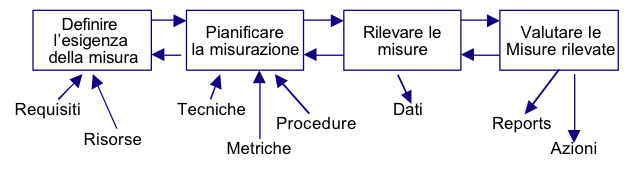
\includegraphics[height=4cm]{img/PQ/pdca.png}
\caption{Ciclo PDCA della misura}
\end{figure}

Nel presente capitolo verranno definite le esigenze di misurazione che si
ritengono necessarie ai fini della qualit\`a, ovvero verr\`a indicato cosa per ogni
singola fase del progetto sar\`a necessario verificare. Verranno indicati gli
strumenti con i quali effettuare la verifica e verranno indicate le metriche con
le quali misurare le propriet\`a di ci\`o che si sta verificando. Verranno
infine indicate le tecniche con le quali procedere. Una volta volta terminata
l'attivit\`a di verifica e la conseguente attivit\`a di misurazione, si proceder\`a con il
riportare l'esito nel capitolo 4 del presente documento. Dopodich\'e, terminata
l'attivit\`a di misurazione, sulla base dei risultati si valuteranno eventuali
decisioni, manovre correttive o l'accettazione del prodotto verificato secondo
le misure e i criteri stabiliti.


\subsection{Verifica della documentazione}

Per ogni documento dovranno essere verificati i seguenti aspetti:
\begin{itemize}
\item correttezza semantica e grammaticale;
\item chiarezza espositiva;
\item assenza di errori concettuali;
\item comprensibilit\`a e accuratezza;
\item correttezza e completezza dei concetti espressi;
\item formattazione del documento secondo quanto specificato dall'amministratore
in\\ \emph{NormeDiProgetto-\versionenormeprogetto.pdf}.
\end{itemize}

Nel caso sia necessario intervenire per correggere uno o pi\`u di questi aspetti
sar\`a dovere del verificatore contattare il redattore del documento affinch\'e
questo gestisca le relative attivit\`a di modifica. Una volta modificato, il
documento dovr\`a essere nuovamente sottoposto all'attenzione del verificatore
per una nuova attivit\`a di verifica.


\subsection{Verifica della fase di analisi}

La fase di analisi dovr\`a essere verificata secondo i seguenti aspetti:

\begin{itemize}

\item scheduling;
\item qualit\`a dei requisiti;
\item completezza del sistema definito rispetto al modello FURPS.
 

\end{itemize}

Il modello FURPS \`e stato elaborato inizialmente da Robert Grady presso i
laboratori dell'Hewlett-Packard. \`E un acronimo mnemonico per la definizione dei requisiti
di software di vario genere e sta a significare:

\begin{itemize}

\item F - Functionality (capacit\`a di fornire le funzioni richieste);
\item U - Usability (facilit\`a d'uso dell'utenza finale);
\item R - Reliability (gestione degli errori e dei crash);
\item P - Performance (Prestazioni);
\item S - Supportability (Supportabilit\`a).
\end{itemize}


Nel caso sia necessario intervenire in maniera correttiva rispetto ad uno o
pi\`u di questi aspetti sar\`a dovere del verificatore contattare l'analista
responsabile affinch\'e provveda alle relative modifiche.



\subsection{Verifica della fase progettuale}

La fase di progettazione dovr\`a essere verificata secondo i seguenti aspetti:

\begin{itemize}

\item soddisfacimento di tutti i requisiti individuati nel documento
\emph{AnalisiDeiRequisiti-\versioneAR.pdf};
\item individuazione di elementi progettuali superflui, non aderenti a nessun
requisito richiesto;
\item corretta corrispondenza e tracciabilit\`a tra i requisiti e le relative
parti del progetto;
\item flessibilit\`a;
\item manutenibilit\`a.

\end{itemize}

Nel caso sia necessario intervenire in maniera correttiva rispetto ad uno o
pi\`u di questi aspetti sar\`a dovere del verificatore contattare il progettista
responsabile affinch\'e provveda alle relative modifiche riguardanti la progettazione.

\subsection{Verifica della fase di realizzazione/programmazione}

La fase di realizzazione/programmazione dovr\`a essere verificata secondo i seguenti aspetti:
\begin{itemize}
\item corretto funzionamento dell'applicazione;
\item affidabilit\`a;
\item efficienza;
\item portabilit\`a;
\item manutenibilit\`a.

\end{itemize}

Nel caso sia necessario intervenire sul codice in base ad uno di questi aspetti
sar\`a dovere del verificatore contattare il programmatore responsabile della
relativa porzione di codice.

Inoltre, per favorire l'attivit\`a di verifica, ogni programmatore sar\`a tenuto
ad eseguire attivit\`a di rilevazione degli errori sul codice per cercare di
diminuire le possibilit\`a d'errore.

\subsection{Validazione}

L'impegno che ci si assume \`e quello di fornire un prodotto completamente e
correttamente funzionante secondo i requisiti concordati. Qualora venissero
riscontrati difetti o non conformit\`a, durante la verifica in fase di collaudo,
ci si impegna ad effettuare modifiche o interventi necessari per risolvere i
problemi.

\section{Risorse necessarie e disponibili}

Per la fase di qualifica sono necessarie risorse di tipo umano che
effettueranno attivit\`a di verifica e validazione cos\`i come definito nel
presente documento. Sono necessarie inoltre risorse di tipo logistico quali
programmi per le attivit\`a di tracciamento tra i requisiti e i moduli software,
un \underline{framework} per i test specifici di unit\`a del codice, un
applicativo software per la gestione e la risoluzione delle anomalie, un ambiente di sviluppo
adeguato con possibilit\`a per i programmatori di rilevare gli errori.


\section{Strumenti}

Per le attivit\`a di verifica ci avvarremo dei seguenti strumenti:

\begin{itemize}

\item Aspell: per controllo ortografico dei
documenti con estensione .tex, necessita di importare un dizionario italiano
(per informazioni \url{http://aspell.net/});

\item JUnit: come unit test framework per il linguaggio di
programmazione \underline{Java} (per informazioni
\url{http://www.junit.org/});

\item Eclipse + \underline{GWT}: per le funzionalit\`a di individuazione e
correzione degli errori di Eclipse su codice Java mentre l'applicazione da
testare verr\`a eseguita in hosted mode tramite GWT (per informazioni \url{http://www.eclipse.org/} e
\url{http://code.google.com/webtoolkit/});

\item Google Project Hosting: per la funzionalit\`a issue-tracker
per la gestione e creazione di ticket cos\`i come descritto nel documento
\emph{NormeDiProgetto-\versionenormeprogetto.pdf} (per informazioni
\url{http://code.google.com/p/netmus/});

\item FindBugs: per effettuare analisi statica del codice
sorgente Java al fine di trovare errori comuni (per informazioni
\url{http://findbugs.sourceforge.net/});

\item PMD \& CPD: per ricercare possibili bug, parti del codice non usate,
espressioni inutili e codice duplicato (per informazioni
\url{http://pmd.sourceforge.net/});

\item CodePro Analytix: per calcolare la misura di varie metriche del
codice sorgente durante la fase di compilazione in modo da tenere continuamente
sotto controllo lo stato del codice stesso (per informazioni
\url{http://code.google.com/intl/it-IT/javadevtools/codepro/doc/index.html});

\item CheckStyle: come aiuto per garantire che il codice Java
aderisca alle pi\`u diffuse norme di codifica (per informazioni
\url{http://checkstyle.sourceforge.net/}).
\end{itemize}


\section{Metriche}

Una metrica viene definita come un metodo di misura associato ad una scala di
valutazione. Secondo il glossario IEEE una metrica \`e la misura quantitativa del
grado con cui un'entit\`a possiede un determinato attributo.

Ai fini della valutazione e quindi di un possibile miglioramento o
correzione della qualit\`a del prodotto finito, devono essere stabilite delle
misure precise con cui misurare quantitativamente i prodotti delle varie fasi
progettuali.


\subsection{Misure nell'analisi dei requisiti}

\begin{itemize}
  
\item Correttezza (se realmente richiesto dal sistema);
\item completezza (se ogni funzione richiesta al software ed il suo
comportamento rispetto ad ogni suo input sono specificati);
\item ambiguit\`a (se ogni requisito ha una sola interpretazione);
\item verificabilit\`a (se \`e possibile verificare che il sistema lo realizzi);
\item consistenza (se nessun requisito \`e in contraddizione con gli altri);
\item tracciabilit\`a (se \`e collegabile a qualche elemento del progetto e del
codice);
\item Function Point (numero di requisiti funzionali).

\end{itemize}


\subsection{Misure nella progettazione}

\begin{itemize}
  
\item Numero di moduli in uno schema di progettazione;
\item livello di coesione tra i moduli;
\item livello di accoppiamento tra moduli.

\end{itemize}


\subsection{Misure sul codice}

\begin{itemize}
  
\item LOC linee di codice;
\item complessit\`a ciclomatica;
\item misure di fan-in e fan-out;
\item misure di complessit\`a;
\item misure object oriented.

\end{itemize}


\subsection{Misure sui test}

\begin{itemize}
  
\item Livello di copertura di istruzioni;
\item livello di copertura dei rami;
\item livello di copertura dei percorsi di base.
\end{itemize}


  
\subsection{Misure sui processi} 

\begin{itemize} 
\item Tempo per le attivit\`a del processo fino al suo completamento;
\item risorse richieste dal processo o dalle sue attivit\`a (ad esempio le
quantit\`a totali di ore/persone).
\item soddisfazione degli Stakeholder.  
\end{itemize}

Qualora la qualit\`a del processo risultasse minore di quella preventivata,
si avranno dei parametri per la stima del costo del miglioramento della qualit\`a
del processo e quindi del prodotto.



\section{Tecniche di Verifica}

L'analisi (verifica) si pone come obiettivo di identificare i difetti presenti nel sistema e in tutte le sue fasi di progettazione.
Essa pu\`o essere divisa in due parti fondamentali:

\begin{itemize}

\item Analisi Statica;
\item Analisi Dinamica. 

\end{itemize}

queste due tecniche verranno approfondite nei successivi paragrafi.


\subsection{Analisi Statica}
Questa forma d'analisi non richiede esecuzione del programma.
Il motivo di ci\`o \`e che eseguire un programma ha un costo che in molti casi
pu\`o portare a preferire controlli basati sulla sola analisi del codice. Si
basa su metodi di lettura, che vengono utilizzati per prodotti semplici, e risulta pi\`u economica poich\'e
l'uso di risorse informatiche \`e limitato.\\ 
Di seguito un elenco dei metodi che abbiamo adottato:


\vspace{1cm}
\begin{table}[h]
\begin{center}
\begin{tabular}{|c|c|}
\hline
\rowcolor{orange}
\bo{Sigla}  & \bo{Descrizione} \\
\hline 
TR & Tracciamento \\ \hline
WT & Walkthrough \\ \hline
IN & Inspection \\ \hline
AFC & Analisi flusso di controllo \\ \hline
AFD & Analisi del flusso di dati \\ \hline
AFI & Analisi del flusso d'informazione \\ \hline
VLC & Verifica corretta logica del codice \\ \hline
VFC & Verifica formale del codice \\ \hline
\end{tabular}
\caption{Tipi di Analisi Statica}
\end{center}
\end{table}

\newpage
\subsubsection*{Tracciamento}

Con il tracciamento si intende mappare l'evoluzione dei requisiti nel corso del
progetto in modo tale da consentire durante le varie fasi di capire quali
requisiti sono stati soddisfatti e quali non ancora o di avere un quadro
generale sullo stato del progetto globale. In fase di progettazione si dovr\`a
controllare che ogni requisito sia implementato correttamente e allo stesso
tempo non esista alcuna funzionalit\`a superflua o componenti inutili. Il
tracciamento deve essere bidirezionale cio\`e esista una
corrispondenza biunivoca tra la fonte e l'oggetto del tracciamento.

\subsubsection*{Walkthrough}

Questa tecnica consiste nella verifica critica dei dati senza
l'assunzione di presupposti e nella simulazione di possibili esecuzioni con l'obiettivo
di rivelare eventuali difetti.

\subsubsection*{Inspection}

Questa tecnica consiste in una verifica mirata dei dati rispettivamente a
determinate metriche con lo scopo di trovare dei tipi precisi di errori.
Prevede la preparazione preliminare del gruppo prima dell'incontro: ogni membro esamina il prodotto, eventualmente applicando tecniche analitiche.

\subsubsection*{Analisi flusso di controllo}

Quest'analisi controlla il codice con lo scopo di determinare se \`e scritto in
modo strutturato e se esegue nel modo desiderato. Controlla inoltre che non ci
sia codice sintatticamente irraggiungibile e cerca parti del codice che possono
portare a terminazioni non desiderate o a cicli infiniti, come chiamate
ricorsive e/o iterazioni.

\subsubsection*{Analisi del flusso di dati}

Accerta che nessun cammino d'esecuzione del programma acceda a variabili prive
di valore, usa i risultati dell'analisi di flusso di controllo insieme alle
informazioni sulle modalit\`a di accesso alle variabili (lettura, scrittura).
Rileva possibili anomalie, per esempio pi\`u scritture successive senza letture
intermedie. \`E complicata dalla presenza e dall'uso di dati globali accedibili
da ogni parte del programma.

\subsubsection*{Analisi del flusso d'informazione}

Quest'analisi va a determinare ed analizzare le dipendenze create tra gli
ingressi e le uscite di un'unit\`a di codice durante la sua esecuzione. Le uniche
dipendenze possibili sono quelle previste dalla specifica, eventuali altre
dipendenze sono da considerarsi errate. Consente inoltre di identificare
eventuali effetti collaterali e pu\`o essere applicata a singoli moduli o a pi\`u
moduli collegati o all'intero sistema.

\subsubsection*{Verifica corretta logica del codice}

Si propone di accertare che il codice sia ben strutturato ed esegua nella
sequenza attesa. Si occupa inoltre di verificare che nessun cammino
d'esecuzione del programma acceda a variabili prive di valore.

\subsubsection*{Verifica formale del codice}

Esplora tutte le esecuzioni possibili mediante prove statiche per rilevare
difetti non sollevati dai test di unit\`a. Si riferisce all'intero sistema integrato.

\subsection{Analisi dinamica}

\subsubsection*{Test di Unit\`a}
Il seguente paragrafo intende illustrare le tecniche utilizzate durante i test
di ogni singola unit\`a.\\ \\
La verifica del codice adotter\`a 2 modelli:

\begin{itemize}
  \item verifica funzionale dei requisiti (Black Box): questo modello si basa su
  un sistema di test a scatola chiusa, ossia partendo dalla conoscenza della struttura interna del 
prodotto, verranno controllati ed accertati che gli output di ogni unit\`a siano  conformi 
a quelli attesi, testandoli in qualunque condizione possibile si possa trovare la singola 
unit\`a. Questi test fanno riferimento alla specifica dell'unit\`a e utilizza
dati in input capaci di provocare in output i dati attesi;
  \item verifica strutturale (White Box): questo modello parte dalla conoscenza 
  delle specifiche del progetto, e come in un sistema a scatola trasparente si analizzano i 
comportamenti specifici dell'unit\`a e dei rispettivi metodi per verificarne la logica 
interna e il corretto funzionamento. In questi test deve essere preso in considerazione 
ogni cammino di esecuzione all'interno del modulo, quindi i casi di prova devono essere 
tutti adeguatamente progettati. 
\end{itemize}


\subsubsection*{Test di Integrazione}
I test d'integrazione rappresentano la logica dei test di unit\`a.
In base al ciclo di vita adottato, ossia il modello incrementale, verranno effettuati dei 
test di integrazione adottando un modello d'integrazione incrementale. 
Non \`e infatti conveniente riunire l'intero sistema e collaudarlo, ma la
strategia utilizzata sar\`a l'integrazione top-down. Ci\`o significa che i
moduli saranno gradualmente integrati in sottosistemi, effettuando opportune verifiche della loro  corretta interazione. 
L'integrazione incrementale top-down richiede l'utilizzo di molti stub che
sostituiscano le componenti; spesso questi stub presentano degli errori dato che sono dei semplici 
prototipi realizzati rapidamente per diminuire i costi, ma permette il funzionamento di 
un sistema parziale molto pi\`u in fretta rispetto ad un modello bottom-up.\\
\\
L'integrazione top-down richiede che ogni componente venga sostituita da uno
stub, a partire dalle foglie nell'albero delle dipendenze, e man mano che si scende si 
inseriscono sempre pi\`u componenti al posto degli stub.

\subsubsection*{Test di Sistema} 
Il test di sistema dovr\`a verifica il comportamento
dinamico del sistema completo rispetto ai requisiti software. Lo scopo \`e
quello di valutare le funzionalit\`a del
prodotto una volta che ha raggiunto la sua completezza.
\\\\ 
La tecnica adottata per verificare l'intero di sistema sar\`a il Test di
Funzionalit\`a, che mira a controllare che ogni funzionalit\`a del
prodotto stabilita dai requisiti sia stata realizzata correttamente.


\section{Metodi di Verifica}

\subsection{Documentazione}

\subsubsection*{Correttezza semantica e grammaticale}

Ispezionare il documento alla ricerca di errori semantici e grammaticali in
tutte le sue parti scritte comprensive di titolo, singoli paragrafi, grafici e didascalie.
Utilizzare la tabella per la correzione dei documenti in appendice a questo
documento.
\\\\
Esito atteso: assenza di errori semantici e grammaticali.
\\\\
Tecniche: WT, IN.

\subsubsection*{Chiarezza espositiva}

Procedere nella lettura del documento facendo attenzione alla forma con cui
sono espressi i concetti. Utilizzare la tabella per la correzione dei documenti
in appendice a questo documento.
\\\\
Esito atteso: linguaggio chiaro e comprensibile privo di ambiguit\`a
d'esposizione.
\\\\
Tecniche: WT.

\subsubsection*{Assenza di errori concettuali}

Procedere nella lettura del documento facendo attenzione al contenuto dei
concetti espressi.\\\\
Esito atteso: assenza di concetti ambigui o in contrasto tra di loro.
\\\\
Tecniche: WT, IN.

\subsubsection*{Comprensibilit\`a e accuratezza}

Verificare il documento nella sua forma e nei contenuti.
\\\\
Esito atteso: assenza di contenuti eccessivamente generici ed interpretabili ai
fini della comprensione.
\\\\
Tecniche: WT, IN.

\subsubsection*{Correttezza e completezza dei concetti espressi}

Verificare il documento soffermandosi su singoli concetti espressi
\\\\
Esito atteso: assenza di concetti incompleti o sbagliati.
\\\\
Tecniche: WT, IN.

\subsubsection*{Correttezza formale}

Verificare il documento soffermandosi sulla correttezza formale delle sue 
singole parti. Utilizzare come riferimento il documento
\emph{NormeDiProgetto-\versionenormeprogetto.pdf} attenendosi alle indicazioni del capitolo 3.
\\\\
Esito atteso: Correttezza formale rispetto a quanto enunciano nelle Norme di
Progetto.
\\\\
Tecniche: WT, IN.


\subsection{Analisi}

\subsubsection*{Qualit\`a dei requisiti}

Verificare la lista di requisiti individuati e indicati nel cap. 5 del documento
\emph{AnalisiDeiRequisiti-\versioneAR.pdf} secondo le metriche nel paragrafo 2.5.1.
Utilizzare la tabella di check per l'analisi qualitativa dei requisiti in
appendice a questo documento.
\\\\
Esito atteso: ogni requisito deve possedere le qualit\`a elencate.
\\\\
Tecniche: WT, IN.


\subsubsection*{Completezza del sistema rispetto al modello FURPS}

Verificare la lista di requisiti individuando per ciascuno a quale requisito
FURPS risponde. Utilizzare la tabella di check per i requisiti FURPS in
appendice a questo documento.
\\\\
Esito atteso: l'insieme dei requisiti individuati deve coprire
efficacemente tutte le specifiche del modello FURPS.
\\\\ Tecniche: IN.

\subsubsection*{Scheduling}

Quantificare il numero di Function Point e sulla base di questi calcolare una
stima della dimensione in LOC del codice. Da questa elaborare una proiezione dei
tempi di programmazione necessari alla realizzazione del software, tenendo in
considerazione che una persona in media si stima riesca ad implementare 12
requisiti funzionali al mese. Per quantificare le linee di codice
rispetto al numero di requisiti funzionali utilizzare come riferimento la
tabella ``Function Point languages table'' reperibile all'indirizzo
\url{http://www.qsm.com/?q=resources/function-point-languages-table/index.html}.
\\\\
Esito atteso: tempistiche adeguate alle possibilit\`a a disposizione.


\subsection{Progettazione ad Alto Livello}

\subsubsection*{Soddisfacimento di tutti i requisiti individuati}

Verificare la corrispondenza dei requisiti individuati in fase di analisi (vedi
cap. 5 del documento \emph{AnalisiDeiRequisiti-\versioneAR.pdf}) con almeno un modulo
software previsto dalla specifica tecnica. Si consiglia di utilizzare la tabella di tracciamento dei requisiti con le relative componenti
software proposta all'interno del documento \emph{SpecificaTecnica-1.0.pdf}.
\\\\
Esito atteso: ci si aspetta di ritrovare all'interno della tabella tutti gli
stessi requisiti cos\`i come individuati in fase di analisi.
\\\\
Tecniche: TR.
\subsubsection*{Individuazione di elementi progettuali superflui}

Individuare tutti i moduli software proposti a livello di progettazione e
verificare che tutti svolgano una funzione richiesta da uno dei requisiti individuati in fase
di analisi. Si consiglia di utilizzare la tabella di tracciamento dei requisiti
con le relative componenti software proposta all'interno del documento
\emph{SpecificaTecnica-1.0.pdf}.
\\\\
Esito atteso: ci si aspetta di ritrovare all'interno della tabella tutti i
moduli software previsti dalla progettazione.
\\\\
Tecniche: TR.

\subsubsection*{Corretta corrispondenza e tracciabilit\`a tra i requisiti e i
moduli software}

Verificare che le funzioni dei moduli software soddisfino le richieste dei
requisiti con cui sono tracciati. Si consiglia di confrontare la descrizione
delle funzionalit\`a fornite dai singoli moduli cos\`i come descritto in
\emph{SpecificaTecnica-1.0.pdf} con la descrizione dei singoli requisiti
proposta nel cap. 5 del documento \emph{AnalisiDeiRequisiti-\versioneAR.pdf}).
\\\\
Esito atteso: ci si aspetta di trovare riscontro tra quello che esigono i
singoli requisiti con le funzionalit\`a descritte dai moduli a loro tracciati.
\\\\
Tecniche: TR, IN.


\subsubsection*{Flessibilit\`a e manutenibilit\`a}

Verificare che il numero di moduli presente sia sufficientemente alto a coprire
in maniera efficace il numero di requisiti funzionali e che tutte le
funzionalit\`a richieste siano distribuite il pi\`u possibile senza incentrare
tutto su pochi moduli costretti a fare tante cose. Controllare la coesione e
l'accoppiamento di ogni singolo modulo. Verificare inoltre la presenza e
l'utilizzo di pattern.
\\\\
Esito atteso: ci si aspetta di trovare un numero di moduli sufficientemente alto
in proporzione al numero di requisiti funzionali. Inoltre ci si aspetta di
rilevare un'alta coesione e un basso accoppiamento di tutti i moduli previsti,
favorito anche dall'utilizzo di un buon numero di pattern. 
\\\\
Tecniche: IN.


\subsection{Progettazione nel Dettaglio}
Nel caso in cui per motivi implementativi ci siano dei
cambiamenti, aggiunta o modifica o eliminazione di qualche modulo, rispetto ai
moduli software preventivati nella \emph{SpecificaTecnica-\versioneST.pdf}, si
dovr\`a rifare tutta la verifica specificata nel paragrafo 2.6.3 di questo
documento, oltre a quella descritta di seguito. 
\subsubsection*{Complessit\`a e riuso}
Verificare il numero di collaborazioni di ogni classe, ovvero con quante classi
\`e accoppiata. L'accoppiamento pu\`o avvenire a seguito di una lettura/modifica
di attributi, di una chiamata di metodi, di una instanziazione di oggetti. \\ \\
Inoltre verificare la coesione di ogni metodo, propriet\`a di un metodo di
accedere in maniera esclusiva ad attributi della classe. Se ogni attributo \`e acceduto da
un solo metodo allora c'\`e massima coesione dei metodi, se i metodi vanno ad
operare sugli stessi attributi allora c'\`e bassa coesione ed \`e difficile
controllare tutte le interazioni tra i metodi dovuti all'uso degli attributi comuni.
\\ \\
Esito atteso: ci si aspetta di trovare un basso accoppiamento tra le classi per
migliorare la modularit\`a e semplificare il riuso, e un alto livello di
coesione dei metodi per semplificare l'architettura delle classi. \\ \\ 
Tecniche: IN.

\subsection{Codifica}

\subsubsection{Verifica Statica}

\subsubsection*{Correttezza delle convenzioni e dello stile}
I verificatori dovranno fare un'attenta lettura del codice ed utilizzare
l'apposito strumento CheckStyle per trovare eventuali errori di non
conformit\`a allo stile, definito chiaramente nelle norme di codifica e
presenti nell'omonima sezione del documento
\emph{NormeDiProgetto-\versionenormeprogetto.pdf}\\\\
Esito atteso: lo stile del codice dovrebbe rispettare le norme stilate a
riguardo e presenti in \emph{NormeDiProgetto-\versionenormeprogetto.pdf}.\\\\ 
Tecniche: WT.

\subsubsection*{Stabilit\`a}
Utilizzare sia lo strumento FindBugs sia lo strumento PMD \& CPD per ricercare
eventuali errori o bug comuni non scovati in precedenza, parti del codice non
usate, cicli inutili e codice duplicato. Ulteriori informazioni sullo strumento
sono riportate nella sezione 2.3.\\\\ 
Esito atteso: ci si aspetta di avere codice pi\`u stabile risolvendo
eventuali errori o elementi inutili trovati.\\\\ 
Tecniche: quelle usate da FindBugs e da PMD \& CPD.

\subsubsection*{Controllo delle metriche e degli indicatori sul codice}
Utilizzare lo strumento CodePro Analytix per misurare:
\begin{itemize}
  \item Lines of Code (numero di linee di codice senza contare spazi e
  commenti): con valore max=\bo{1600} per unit\`a di compilazione;
  \item Number of Types (numero di classi e di interfacce in un package): con
  valore max=\bo{30} per package;
  \item Afferent Couplings (valore di fan-in);
  \item Efferent Couplings (valore di fan-out): con valore max=\bo{20};
  \item Number of Methods (numero di metodi): con valore max=\bo{60} per Type;
  \item Number of Methods Per Type (numero di metodi per ogni
  classe/interfaccia): con valore max=\bo{15};
  \item Number of Parameters (numero di parametri per
  metodo): con valore max=\bo{6};
  \item Lines Of Code Per Method (numero di linee di codice
  per metodo): con valore max=\bo{40};
  \item Block Depth (grado di annidamento per metodo): con valore max=\bo{4};
  \item Cyclomatic Complexity (complessit\`a ciclomatica): con valore max=\bo{10}.
\end{itemize}
Questo tool permette di evidenziare eventuali package o classi che
potrebbero essere particolarmente complicati, o scritti in modo confuso.
Ulteriori informazioni sullo strumento sono riportate nella sezione 2.3.\\\\ 
Esito atteso: i valori misurati sia nei package sia nei metodi delle
classi, dovrebbero essere nella norma.\\\\ 
Tecniche: quelle usate da CodePro Analytix.

\subsubsection{Verifica Dinamica}

\subsubsection*{Test di Unit\`a}

Alcuni test di unit\`a creati e poi eseguiti, dovranno  avere il
compito di testare le funzionalit\`a base del metodo della classe indicato,
altri avere il compito di testare la struttura del metodo ed altri ancora la
correttezza del metodo con casi limite. Inoltre molti test dovranno essere
effettuati su metodi set/get per verificare la corretta comunicazione tra di loro. Per tutti i test si dovr\`a adottare il framework
JUnit, ritenuto il pi\`u attendibile tra i framework messi a disposizione nella
rete, oltre ad essere integrato in Eclipse e a permettere una netta separazione
tra codice e test.
\\\\
Il piano dei test di unit\`a (che dovr\`a essere chiaramente esposto al termine
della progettazione in dettaglio) sar\`a presente in appendice E e preveder\`a
che per ogni test siano elencati:
\begin{itemize}
  \item unit\`a o modulo su cui sar\`a effettuato il test;
  \item obiettivo del test;
  \item strategia adottata;
  \item tipologia (whitebox o blackbox);
  \item aspettative.
\end{itemize}

I risultati dei test saranno presenti in appendice A.2 ed elencati in
questo modo:
\begin{itemize}
  \item unit\`a o modulo su cui \`e stato effettuato il test;
  \item esito del test;
  \item malfunzionamenti rilevati.
\end{itemize}

L'obiettivo \`e quello di rintracciare tutti gli errori presenti all'interno del
codice ed una volta identificati, risolverli. Da sottolineare che come afferma la tesi di Dijkstra 
i test non possono dimostrare la totale assenza di errori.


\subsubsection*{Test di Integrazione} 
Applicando la tecnica top-down per
l'integrazione incrementale, si dovranno sviluppare prima le parti pi\`u
esterne, quelle poste sulle foglie dell'albero delle dipendenze e poi si dovr\`a
scendere.
\\\\
Lo schema da seguire \`e il seguente:
\begin{itemize}
  \item si progetta, scrive e testa una parte del sistema;
  \item se ne scrive un altro pezzo;
  \item si integrano le due parti e si testa;
  \item ogni malfunzionamento rilevato sar\`a conseguenza del malfunzionamento
  dell'ultima componente aggiunta.
\end{itemize}

Il piano dei test di integrazione sar\`a presente in appendice F e preveder\`a
che per ogni test siano elencati:
\begin{itemize}
  \item classi coinvolte nel test;
  \item obiettivo del test;
  \item strategia adottata;
  \item aspettative.
\end{itemize}

I risultati dei test saranno presenti in appendice A.2 ed elencati in
questo modo:
\begin{itemize}
  \item classi coinvolte nel test;
  \item esito del test;
  \item malfunzionamenti rilevati.
\end{itemize}

\subsubsection*{Test di Sistema}
Lo scopo di questo test \`e quello di verificare il comportamento dinamico del
sistema completo rispetto ai requisiti software e valutare le funzionalit\`a del
prodotto.
\\\\
La tecnica adottata sar\`a il Test di Funzionalit\`a che insieme al tracciamento
dei requisiti presente in \emph{AnalisiDeiRequisiti-\versioneAR.pdf},
permetter\`a di verificare che effettivamente tutti i requisiti software siano
soddisfatti. Per ogni requisito si dovr\`a controllare che sia stato
implementato e presente nel prodotto, e che svolga le funzionalit\`a richieste.


% INIZIO CAPITOLO 3

\chapter{Gestione amministrativa della \\revisione}
\thispagestyle{fancy} % per lo stile di header e footer

\section{Comunicazione e risoluzione di anomalie}

Un'anomalia \`e una deviazione da una norma o da una struttura standard
considerata normale. Possiamo prevedere che la maggioranza delle anomalie verr\`a 
rilevata durante il processo di verifica. Nonostante i verificatori svolgano un
ruolo fondamentale nel trattamento delle anomalie, non possiamo escludere che
queste vengano riscontrate anche durante una qualsiasi fase di ciclo di vita,
quindi non vogliamo limitare il compito della comunicazione ai soli verificatori ma 
intendiamo estendere il caso a tutti i membri del gruppo di lavoro.

\subsection{Comunicazione}

Per notificare anomalie dovr\`a essere usato lo strumento issue-tracker messo a
disposizione nella pagina \url{http://code.google.com/p/netmus/}. Per ogni
anomalia individuata si dovr\`a creare un ticket. Per la creazione e la struttura dei
singoli ticket fare riferimento al documento \emph{NormeDiProgetto-\versionenormeprogetto.pdf} paragrafo omonimo.


\subsection{Gestione dell'anomalia}

Il verificatore che individua un'anomalia dovr\`a innanzitutto analizzare il
problema per valutare la causa dell'anomalia.
In seguito verr\`a comunicato, a chi ne ha competenza, il tipo e l'ubicazione
dell'errore, allegando una descrizione chiara del problema ed elencando le
cause. L'incaricato dovr\`a provvedere ad una possibile soluzione. Se il
problema fosse particolarmente grave, sar\`a necessario un incontro con i membri 
del gruppo per cercare una soluzione. Una volta risolto, il modulo viene
riverificato.

\section{Trattamento delle discrepanze}

Una discrepanza \`e un discostamento, totale o parziale, dalle attese del
committente o del gruppo stesso, rilevabile in un prodotto intermedio
o finale. \`E compito dei verificatori, una volta individuata una discrepanza,
comunicarlo al gruppo tramite l'apertura di un ticket. Per notificare una
discrepanza dovr\`a essere usato lo strumento issue-tracker messo a disposizione nella pagina \url{http://code.google.com/p/netmus}. 
Esso dovr\`a avere struttura simile a quella indicata nel
documento \emph{NormeDiProgetto-\versionenormeprogetto.pdf}, ma la priorit\`a assegnatagli dovr\`a essere quella
massima. I verificatori analizzeranno il problema usando la tabella di
tracciabilit\`a dei requisiti. Verr\`a trovato quale o quali di questi problemi non
rispettano le aspettative del cliente o, in alternativa, quale requisito non \`e
stato rispettato. Se il problema fosse risolvibile in tempi e costi ragionevoli
l'impegno sar\`a focalizzato nella soluzione di quest'ultimo. Altrimenti si dovr\`a
redarre un documento da consegnare al cliente con la descrizione accurata della
discrepanza.\\

Vanno incluse:

\begin{itemize}

\item eventuali responsabilit\`a;
\item il preventivo dei tempi e dei costi necessari alla risoluzione;
\item una lista dei requisiti non soddisfatti.

\end{itemize}

In seguito si potranno prendere eventuali accordi con il cliente. In caso
contrario il progetto sar\`a esposto ad alto rischio di fallimento.

\section{Procedure di controllo di qualit\`a di processo}
Per ogni processo di verifica verr\`a aperto un ticket (per maggiori dettagli vedi
``Pianificazione, ticketing e time-tracking'' in \emph{NormeDiProgetto-\versionenormeprogetto.pdf}). Dopo aver
accettato la commessa ogni verificatore dovr\`a verificare le caratteristiche di
qualit\`a stabilite nel capitolo 2 del presente documento applicando le tecniche
appropriate e i relativi metodi di misurazione. A lavoro terminato il
verificatore dovr\`a redarre un resoconto valutando i dati raccolti rispetto agli
esiti predetti.

\subsection{Test di valutazione sul processo di lavoro}
Per una chiara comprensione su come alcuni fattori possono influenzare le varie
fasi del progetto e per ricercare un miglioramento del processo \`e
stato introdotto un sistema di feedback su tutte le attivit\`a svolte.\\ \\
Alla chiusura di un ticket, chi ha effettuato il lavoro deve compilare un form
contenente un test di valutazione sui seguenti aspetti:

\begin{itemize}
\item lavoro svolto;
\item interazione con gli altri;
\item strumenti utilizzati;
\item tempo impiegato.
\end{itemize}

La valutazione \`e assegnata su una scala numerica da 1 a 10 in modo crescente
rispetto al proprio livello di soddisfacimento.
In prossimit\`a di una revisione e prima della consegna verranno sviluppati
quattro grafici per rappresentare i dati raccolti rispetto gli ambiti. 
I risultati ottenuti confrontati con le valutazioni ricevute in seguito nella
fase di revisione potranno fornire interessanti spunti su come correggere o
rafforzare il metodo di lavoro.




% INIZIO CAPITOLO 5

\chapter{Pianificazione ed esecuzione del \\collaudo}
\thispagestyle{fancy} % per lo stile di header e footer

\section{Specifica della campagna di validazione \\(collaudo incluso)}
Durante la fase di collaudo, si attuer\`a un procedimento per individuare carenze
relative alla correttezza, alla completezza e all'affidabilit\`a delle componenti 
software create rispetto ai requisiti definiti durante la fase di analisi.\\ \\
Il collaudo consister\`a in due fasi: 

\begin{itemize}
  \item collaudo interno(alpha test): viene effettuato prima del rilascio
  del prodotto internamente al gruppo e consiste in verifica finale del tracciamento 
  e in prove di esecuzione, anche se quest'ultime non sono da considerarsi tecniche di
  ricerca e risoluzione di errori.
  \item collaudo esterno(beta test): viene effettuato una volta superato il
  collaudo interno. Durante questo test il prodotto viene rilasciato a
  pochi utenti esterni i quali vengono avvertiti che il prodotto potrebbe non essere 
  di qualit\`a elevata e avere bisogno di ulteriori correzioni. 
  Il compito di questi soggetti esterni e di valutarne la fruibilit\`a e l'accessibilit\`a.
\end{itemize}

Una volta che il prodotto sar\`a completato, tutti i requisiti dovranno essere
stati soddisfatti.\\
\\
Di seguito riportiamo una tabella che riporta requisiti tracciati e metodi per
la verifica nel prodotto finale.

\begin{table}
\begin{center}
\begin{tabular}{|p{0.32\textwidth}|p{0.32\textwidth}|p{0.30\textwidth}|}
\hline
\bo{Gruppo}\cellcolor{orange}& \bo{Requisito}\cellcolor{orange}& \bo{Metodo
di Verifica}\cellcolor{orange}
\\
\hline

\bo{A} &
\bo{C1FN-1.1, C1FN-1.1.2, C1FN-1.1.3, C1FD-1.1.4,
C1FN-1.3, C1FO-1.3.3, C1FO-1.3.4, C1FD-1.4.4, C1FD-1.5,
C1FD-1.7, C1FD-1.7.1, C1FO-1.7.2 } & Questi
requisiti potranno essere verificati tramite l'utilizzo della GUI messa a
disposizione dell'utente. \\ \hline
\bo{B} &
\bo{C1FN-1.2, C1FN-1.2.1, C1FN-1.3.1,
C1FN-1.4, C1FN-1.4.1, C1FN-1.4.2}   & Tali requisiti saranno verificati tramite
l'utilizzo della GUI con rispettivi controlli sul Database per
verificare che le modifiche effettuate siano state registrate correttamente.
\\\hline 
\bo{C} &
\bo{C1FD-1.3.2, C1FN-1.4.3} & Questi requisiti
potranno essere verificati tramite il solo controllo del Database. \\ \hline
\bo{D} &
\bo{C1FO-1.8.1} & Il requisito potr\`a essere verificato qualora l'esportazione e
la creazione del PDF abbiano successo. \\\hline
\bo{E} & 
\bo{C1FD-1.10, C2FD-2} & Tali requisiti potranno essere verificati nel momento
in cui la periferica USB risulter\`a aggiornata. \\\hline
\bo{F} &
\bo{C2FN-1, C2FN-1.1, C2FN-1.2, C2FD-1.4, C2FN-1.5, C2FN-3, C2FN-3.1}& Questi
requisiti riguardano la componente C2. La loro verifica consister\`a
nell'apparizione di messaggio di avviso sulla DEVICE SCANNER BAR
all'interno della view.\\\hline
\end{tabular}
\caption{Gruppi di requisiti e rispettivi metodi di verifica in fase di
collaudo}
\end{center}
\end{table}

Presentiamo ora una descrizione delle prove che intendiamo proporre al
committente per il collaudo del prodotto. \\
La validazione delle funzionalit\`a soddisfatte dai requisiti seguir\`a le
metodologie qui proposte col prodotto ultimato.

\begin{itemize}
  \item Requisito C1FN-1.2.1 : Pagina di Login\\
  \\Per validare tale requisito basta solamente accedere alla pagina
  iniziale di NetMus. Qui verr\`a presentata da subito l'interfaccia per il
  login del sistema NetMus. I Sistemi di Login offerti sono 2: NetMus Login e
  Google Login, oltre all'interfaccia di registrazione a NetMus.
  
  \item Requisito C1FN-1.2 : Registrazione\\
  \\Il Sistema Netmus offre la possibilit\`a di registrarsi qualora non si sia
  iscritti. Basta cliccare sulla pagina di login la voce ``Sign up to
  NetMus''. Qui \`e necessario inserire un'email valida e la password.
  
  \item Requisiti C1FN-1.1, C1FN-1.1.1, C1FN-1.1.2, C1FD-1.1.4, C1FO-1.3.4,
  C1FD-1.5 :\\
  Grafica simile ad iTunes, Elenco brani, Menu laterali, Player
  YouTube, Ranking brani, Riproduzione tracce in streaming\\
  \\Effettuare  l'accesso a NetMus per validare questo requisito. La ProfileView
  ci mostra da subito la grafica del sistema, con menu laterali e l'elenco dei brani della libreria dell'utente. Inoltre il player di youtube
  \`e gi\`a presente nella pagina, basta selezionare con un click la canzone che
  si vuole ascoltare e successivamente premere sul tasto ``Play'' per la
  riproduzione e la visualizzazione del video. A fianco della finestra in cui
  compare la riproduzione della canzone in streaming \`e presente la voce ``dai
  il tuo voto'' e cliccando sul numero di stelline che si desidera
  assegnare alla canzone  \`e possibile esprimere un giudizio.
  
  \item Requisito C1FN-1.1.3 : Informazioni dettagliate brano\\
  \\Dalla pagina di visualizzazione brani \`e possibile accedere alle
  informazioni dettagliate su un brano semplicemente con un doppio click sul brano
  desiderato, si aprir\`a una nuova finestrella con le informazioni del brano e
  la relativa copertina e voto.
  
  \item Requisito C1FN-1.3.1, C1FN-1.3.2 : Modifica informazioni brano,
  Cancellazione brano\\
  \\Dalla view del Profilo, selezionando una canzone e successivamente cliccando
  sul tasto ``Edit Songs'' sar\`a possibile modificare le informazioni di un
  brano, oppure cancellare il brano stesso.
  
  \item Requisito C1FO-1.3.3 : Creazione playlist\\
  \\Nel menu laterale a sinistra, alla voce playlist saranno elencate le
  playlist dell'utente. Cliccando il tasto ``+'' \`e possibile creare una nuova playlist
  in cui inserire i brani che si desidera avere nella suddetta playlist.
  
  \item Requisiti C1FN-1.4, C1FN-1.4.1, C1FN-1.4.2 : Gestione profilo personale,
  Modifica informazioni personali, Cambio password\\ 
  \\Cliccando il tasto ``account" sulla
  view del profilo \`e possibile inserire informazioni aggiuntive riguardanti il proprio profilo, oppure modificare i
  propri dati, compreso l'inserimento di una nuova password.
  
  \item Requisiti C1FO-1.8.1 : Esportazione pdf\\
  \\Per esportare la propria libreria musicale in pdf basta cliccare
  semplicemente sul tasto ``esporta pdf'' presente in basso a destra e il pdf verr\`a creato
  automaticamente, permettendo il salvataggio nella directory che si preferisce.
  
  \item C1FD-1.8 : Elaborazione dati utente\\
  \\Per visualizzare statistiche e altre svariate informazioni sulla propria
  libreria basta cliccare sul tasto in basso a sinistra ``statistiche'', si aprir\`a una
  nuova finestra con elencate tutte le informazioni statistiche.
  
  \item C2FN1, C2FN-1.1, C2FN-1.2, C2FN-1.4, C2FN-1.5, C2FD-2, C2FN-3,
  C2FN-3.1 :\\
  Recupero delle informazioni, Recupero automatico, Recupero
  manuale, Informazioni dall'hard disk, File ignorati, C2FD-2 Aggiornamento e
  completamento informazioni, Comunicazione con C1, Invio delle informazioni\\
  \\A fianco della libreria personale \`e presenta una barra ``Device Scanner
  BAR'' a scomparsa. Basta passarci sopra con il cursore per visualizzarla. Tale
  barra implementa la componente di recupero delle informazioni. 
  Inserendo un qualunque dispositivo di archiviazione in una porta
  USB del PC, la componente di recupero lo individua e ne analizza il
  contenuto, estraendo tutte le informazioni dei file mp3 e monitorando il
  progresso dell'operazione che diventa visibile all'utente. La
  scansione pu\`o essere fatta anche manualmente cliccando sul tasto ``Scan
  Folder'' e selezionando una directory qualunque del PC. Le informazioni vengono automaticamente inviate alla 
  componente di persistenza che li inserisce nel catalogo. Se le canzoni sono
  gi\`a presenti nel database queste vengono inserite solamente nel catalogo
  dell'utente e, qualora le informazioni fossero incomplete, vengono completate
  con quelle della medesima canzone gi\`a presente nel catalogo. La funzione di
  completamento delle info oltre a controllare nel proprio database, fa
  riferimento anche a servizi esterni, anche per la ricerca delle copertine
  degli album. \`E possibile anche disabilitare la lettura automatica dei
  dispositivi di massa inseriti cliccando la voce ``disable'' sempre nella Device Scanner BAR.
  
\end{itemize}


\section{Dettaglio dell'esito della campagna di validazione}
------TEST UNITA e TEST INTEGRAZIONE ??????------////

\subsection{Test di Sistema}

\subsubsection{Test alpha}
L'esito sul test alpha v.0.1, collaudo interno fatto sul software non appena
tutto il sistema era pronto e verificato tramite i vari test di unit\`a e di
integrazione, ha avuto un esito positivo in quanto ha dimostrato che tutti i
requisiti obbligatori pattuiti nell'analisi dei requisiti sono stati rispettati.
\begin{footnotesize}
\begin{longtable}{|p{2,4cm}|p{2,4cm}|}
\hline
\rowcolor{orange} \bo{Requisito}  & \bo{Presenza} \\
\hline
\endhead
\hline
\multicolumn{2}{|c|}{\textit{continua alla pagina successiva}}\\
\hline
\endfoot
\endlastfoot
 C1FN-1 &X \\ \hline
 C1FN-1.1 &X  \\ \hline
 C1FN-1.1.1 &X  \\ \hline
 C1FN-1.1.2  &X  \\ \hline
 C1FN-1.1.3 &X  \\ \hline
 C1FN-1.2 &X  \\ \hline
 C1FN-1.2.1 &X  \\ \hline
 C1FN-1.3 &X  \\ \hline
 C1FN-1.3.1  &X  \\ \hline
 C1FN-1.4 &X  \\ \hline
 C1FN-1.4.1 &X  \\ \hline
 C1FN-1.4.2 &X  \\ \hline
 C1FN-1.4.3 &X  \\ \hline
 C1FN-1.9 &X  \\ \hline
 C1FN-1.9.1  &X  \\ \hline
 C1FN-1.9.2 &X  \\ \hline
 C1FN-1.9.5 &X  \\ \hline
 C1FN-1.13 &X  \\ \hline
 C1QN-1.9.4 &X  \\ \hline
 C1QN-1.9.6 &X  \\ \hline
 C1QN-1.6 &X \\ \hline
 C1QN-1.6.2&X   \\ \hline
 C1QN-2&X \\ \hline
 C1QN-2.3&X  \\ \hline
 C1QN-2.6&X  \\ \hline
 C1QN-2.7&X    \\ \hline
 C1QN-3.1&-   \\ \hline
 C1VN-1.12&X \\ \hline
 C1VN-1.13.1&X  \\ \hline
 C1VN-1.11&X  \\ \hline
 C1VN-2.2&- \\ \hline
 C1VN-2.5&X  \\ \hline
 C2FN-1&X    \\ \hline
 C2FN-1.1&X    \\ \hline
 C2FN-1.2&X   \\ \hline
 C2FN-1.5&X   \\ \hline
 C2FN-3&X   \\ \hline
 C2FN-3.1&X   \\ \hline
 C2QN-3.2&X   \\ \hline
 C2QN-4 &X  \\ \hline
 C2QN-4.4&X  \\ \hline
 C2VN-4.6&X    \\ \hline
 C2VN-4.7&-  \\ \hline
\caption{Check sulla presenza dei requisiti obbligatori nel test alpha v.0.1}
\end{longtable}
\end{footnotesize}
I tre requisiti non presenti all'interno del prodotto nel test alpha, sono i
requisiti sulla licenza open-source del prodotto e sulla presenza del manuale utente.
Questi requisiti sono comunque stati rispettati. Pertanto non si procede a
rilasciare una nuova versione del prodotto per il test alpha.

\subsubsection{Test beta}
Dopo aver superato il test alpha, si \`e proseguito rilasciando il prodotto ad
un campione di 8/10 persone, di cui una \`e il prof. Riccardo Cardin, in una
versione beta 0.1. Dopo aver aspettato alcuni giorni e un numero consistente di
feedback, il resoconto dei problemi \`e:
\begin{itemize}
  \item mancanza di una pagina di Credits, dove reperire le varie informazioni
  del sistema (esempio: versione rilasciata del prodotto); 
  \item mancanza di una pagina di Help, dove poter consultare eventuali
  problematiche che si presentano;
  \item mancanza di un Contact, per poter comunicare eventuali problemi o
  per contattare l'amministratore del sistema;
  \item alcuni bottoni non collegati a link;
  \item nelle playlist manca la possibilit\`a di ordinare a proprio piacimento
  le canzoni;
  \item problemi se inserisco delle canzoni che hanno dei caratteri cinesi o
  giapponesi nei titoli;
  \item a volte dopo aver inserito delle nuove canzoni serve un refresh manuale
  della pagina per far s\`i che compaiano nella lista;
  \item ambiguit\`a nell'uso dei pulsanti a forma di X rossa, alcune volte serve
  per chiudere un pop-up altre per togliere una canzone dalla playlist;
  \item mancanza delle funzionalit\`a Social Network del sistema, non c'\`e la
  possibilit\`a di visualizzare il profilo di altri utenti.
\end{itemize}
Alcuni di questi problemi son stati risolti dato che ero requisiti obbligatori,
mentre quelli desiderabili/opzionali come ----------- si \`e deciso di non
implementarli.
La beta \`e passata alla versione 0.2 e distribuita alla stessa utenza.



\listoftables
\addcontentsline{toc}{chapter}{Indice Tabelle}
\listoffigures
\addcontentsline{toc}{chapter}{Indice Figure}



\appendix


\chapter{Resoconto delle attivit\`a di verifica}
\thispagestyle{fancy} % per lo stile di header e footer

\section{Dettaglio delle verifiche tramite analisi}

\subsection{Verifica sull'Analisi}

\subsubsection*{Qualit\`a dei Requisiti}

Verifica dei requisiti proposti nel documento
\emph{AnalisiDeiRequisiti-1.6.pdf}.

\begin{footnotesize}
\begin{longtable}{|p{2,4cm}|p{1,8cm}|p{1,8cm}|p{1,8cm}|p{1,8cm}|p{1,8cm}|p{1,8cm}|}
\hline
\rowcolor{orange} \bo{Requisito}  & \bo{Corr.}  & \bo{Comp.}  &
\bo{Ambi.} & \bo{Veri.}  & \bo{Cons.}  & \bo{Trac.}
\\
\hline
\endhead
\hline
\multicolumn{7}{|c|}{\textit{continua alla pagina successiva}}\\
\hline
\endfoot
\endlastfoot
 
 C1FN-1& OK&  OK&  OK&  OK&  OK& -\\ \hline
 C1FN-1.1&  OK&  OK&  debole&  OK&  OK& OK\\ \hline
 C1FN-1.1.1&  OK&  OK&  OK&  OK&  C1FN-1.3& OK\\ \hline
 C1FN-1.1.2&  OK&  OK&  OK&  OK&  OK& OK\\ \hline
 C1FN-1.1.3&  OK&  OK&  OK&  OK&  OK& OK\\ \hline
 C1FD-1.1.4&  OK&  OK&  OK&  OK&  OK& OK\\ \hline
 C1FN-1.2&  OK&  OK&  OK&  OK&  OK& OK\\ \hline
 C1FN-1.2.1&  OK&  OK&  OK&  OK&  OK& OK\\ \hline
 C1FN-1.3&  OK&  debole&  debole&  OK&  C1FN-1.1.1& OK\\ \hline
 C1FN-1.3.1&  OK&  OK&  OK&  OK&  OK& OK\\ \hline
 C1FD-1.3.2& OK&  OK&  ambiguo&  OK&  OK& OK\\ \hline
 C1FO-1.3.3&  OPZ.&  OK&  OK&  OK&  OK& OK\\ \hline
 C1F0-1.3.4&  OPZ.&  OK&  OK&  OK&  OK& OK\\ \hline
 C1FN-1.4&  OK&  OK&  OK&  OK&  OK& OK\\ \hline
 C1FN-1.4.1&  OK&  OK&  OK&  OK&  OK& OK\\ \hline
 C1FN-1.4.2&  OK&  OK&  OK&  OK&  OK& OK\\ \hline
 C1FN-1.4.3&  OK&  OK&  OK&  OK&  OK& OK\\ \hline
 C1FD-1.4.4&  OK&  OK&  OK&  OK&  OK& OK\\ \hline
 C1FD-1.5&  OK&  OK&  OK&  OK&  OK& OK\\ \hline
 C1FD-1.7&  OK&  OK&  OK&  OK&  OK& OK\\ \hline
 C1FD-1.7.1&  OK&  OK&  OK&  OK&  OK& OK\\ \hline
 C1F0-1.7.2&  OPZ.&  OK&  OK&  OK&  OK& OK\\ \hline
 C1FD-1.8&  OK&  OK&  OK&  OK&  OK& -\\ \hline
 C1F0-1.8.1&  OPZ.&  OK&  OK&  OK&  OK& OK\\ \hline
 C1FN-1.9&  OK&  OK&  OK&  OK&  OK& -\\ \hline
 C1FN-1.9.1&  OK&  OK&  OK&  OK&  OK& -\\ \hline
 C1FN-1.9.2&  OK&  OK&  OK&  OK&  OK& -\\ \hline
 C1FN-1.9.5&  OK&  OK&  OK&  OK&  OK& -\\ \hline
 C1FO-1.9.3&  OPZ.&  OK&  OK&  OK&  OK& -\\ \hline
 C1FD-1.10&  OK&  OK&  OK&  OK&  OK& OK\\ \hline
 C1FN-1.13&  OK&  OK&  OK&  OK&  OK& OK\\ \hline
 C1QD-1.5.1&  OK&  OK&  OK&  OK&  OK& -\\ \hline
 C1QN-1.9.4&  OK&  OK&  OK&  OK&  OK& -\\ \hline
 C1QN-1.9.6&  OK&  OK&  OK&  OK&  OK& -\\ \hline
 C1QN-1.6&  OK&  OK&  OK&  OK&  OK& -\\ \hline
 C1QD-1.6.1&  OK&  OK&  OK&  OK&  OK& -\\ \hline
 C1QN-1.6.2&  OK&  OK&  OK&  debole&  OK& -\\ \hline
 C1QN-2&  OK&  OK&  OK&  OK&  OK& -\\ \hline
 C1QO-2.1&  OPZ.&  OK&  OK&  OK&  OK& -\\ \hline
 C1QN-2.3&  OK&  OK&  OK&  OK&  OK& -\\ \hline
 C1QD-2.4&  OK&  OK&  OK&  OK&  OK& -\\ \hline
 C1QN-2.6&  OK&  OK&  OK&  OK&  OK& -\\ \hline
 C1QN-2.7&  OK&  OK&  OK&  OK&  OK& -\\ \hline
 C1QN-3.1&  OK&  OK&  OK&  OK&  OK& -\\ \hline
 C1QD-3.1.1&  OK&  OK&  OK&  OK&  OK& -\\ \hline
 C1VN-1.12&  OK&  OK&  OK&  OK&  OK& -\\ \hline
 C1VN-1.13.1&  OK&  OK&  OK&  OK&  OK& -\\ \hline
 C1VN-1.11&  OK&  OK&  OK&  OK&  OK& -\\ \hline
 C1VD-1.5.2&  OK&  OK&  OK&  OK&  OK& -\\ \hline
 C1VD-1.5.3&  OK&  OK&  OK&  OK&  OK& -\\ \hline
 C1VN-2.2&  OK&  OK&  OK&  OK&  OK& -\\ \hline
 C1VN-2.5&  OK&  OK&  OK&  OK&  OK& -\\ \hline
 C2FN-1&  OK&  OK&  OK&  OK&  OK& OK\\ \hline
 C2FN-1.1&  OK&  OK&  OK&  OK&  OK& OK\\ \hline
 C2FN-1.2&  OK&  OK&  OK&  OK&  OK& OK\\ \hline
 C2FO-1.3&  OK&  OK&  OK&  OK&  OK& -\\ \hline
 C2FD-1.4&  OK&  OK&  OK&  OK&  OK& OK\\ \hline
 C2FN-1.5&  OK&  OK&  OK&  OK&  OK& OK\\ \hline
 C2FO-1.6&  OPZ.&  OK&  OK&  OK&  OK& -\\ \hline
 C2FD-2&  OK&  OK&  OK&  OK&  OK& OK\\ \hline
 C2FN-3&  OK&  OK&  OK&  OK&  OK& OK\\ \hline
 C2FN-3.1&  OK&  OK&  OK&  OK&  OK& OK\\ \hline
 C2QD-1.7&  OK&  OK&  OK&  OK&  OK& -\\ \hline
 C2QN-3.2&  OK&  OK&  OK&  OK&  OK& -\\ \hline
 C2QN-4&  OK&  OK&  vago&  OK&  C2QD-4.2& -\\ \hline
 C2QD-4.1&  OK&  OK&  OK&  OK&  OK& -\\ \hline
 C2QD-4.2&  OK&  OK&  OK&  OK&  C2QN-4& -\\ \hline
 C2QD-4.3&  OK&  OK&  OK&  OK&  OK& -\\ \hline
 C2QN-4.4& OK&  OK&  OK&  OK&  OK& -\\ \hline
 C2VD-4.5&  OK&  OK&  OK&  OK&  OK& -\\ \hline
 C2VN-4.6&  OK&  OK&  OK&  OK&  OK& -\\ \hline
 C2VN-4.7&  OK&  OK&  OK&  OK&  OK& -\\ \hline
 
\caption{Check sulla qualit\`a dei requisiti (AnalisiDeiRequisiti-1.6.pdf)}
\end{longtable}
\end{footnotesize}

Dall'analisi dei requisiti sono emerse in particolar modo due inconsistenze. La
prima coinvolge la componente C1FN-1.3 e la componente C1FN-1.1.1 che pur non
essendo in evidente contrasto a fronte di un'interpretazione scorretta dovuta
all'ambiguit\`a rilevata in C1FN-1.3 potrebbero risultarlo.
La seconda riguarda C2QD-4.2 e C2QN-4. Anche queste pi\`u che in contraddittorio
sembrano coprire, se pur con una diversa sfumatura, la stessa esigenza.
\\\\
Requisiti sistemati nel documento \emph{AnalisiDeiRequisiti-1.8.pdf} a fronte
della verifica della versione 1.7.
\\\\
Verifica dei requisiti proposti nel documento \emph{AnalisiDeiRequisiti-1.8.pdf}

\begin{footnotesize}
\begin{longtable}{|p{2,4cm}|p{1,8cm}|p{1,8cm}|p{1,8cm}|p{1,8cm}|p{1,8cm}|p{1,8cm}|}
\hline
\rowcolor{orange} \bo{Requisito}  & \bo{Corr.}  & \bo{Comp.}  &
\bo{Ambi.} & \bo{Veri.}  & \bo{Cons.}  & \bo{Trac.}
\\
\hline
\endhead
\endfoot
 C1FN-1.3&  OK&  OK&  OK&  OK&  OK & OK\\ \hline
 C2QD-4.2&  OK&  OK&  OK&  OK&  OK& -\\ \hline
\caption{Check sulla qualit\`a dei requisiti (AnalisiDeiRequisiti-1.8.pdf)}
\end{longtable}
\end{footnotesize}

Dall'analisi dei requisiti indicati risultano corretti i problemi
d'inconsistenza emersi precedentemente. 


\subsubsection*{Completezza dei requisiti rispetto al modello FURPS}

Verifica dei requisiti proposti nel documento
\emph{AnalisiDeiRequisiti-1.6.pdf}.


\begin{footnotesize}
\begin{longtable}{|p{2,4cm}|p{0,7cm}|p{0,7cm}|p{0,7cm}|p{0,7cm}|p{0,7cm}|}
\hline
\rowcolor{orange} \bo{Requisito}  & \bo{F.}  & \bo{U.}  & \bo{R.}  & \bo{P.}  &
\bo{S.}  \\
\hline
\endhead
\hline
\multicolumn{6}{|c|}{\textit{continua alla pagina successiva}}\\
\hline
\endfoot
\endlastfoot
 
 C1FN-1& X&  X&  &  &  \\ \hline
 C1FN-1.1& X&  X&  &  &  \\ \hline
 C1FN-1.1.1& X&  &  &  &  \\ \hline
 C1FN-1.1.2& X&  X&  &  &  \\ \hline
 C1FN-1.1.3& X&  &  &  &  \\ \hline
 C1FD-1.1.4& X&  &  &  &  \\ \hline
 C1FN-1.2& X&  &  &  &  \\ \hline
 C1FN-1.2.1& X&  &  &  &  \\ \hline
 C1FN-1.3& X&  X&  &  &  \\ \hline
 C1FN-1.3.1& X&  &  &  &  \\ \hline
 C1FD-1.3.2& X&  &  &  &  \\ \hline
 C1FO-1.3.3& X&  X&  &  &  \\ \hline
 C1F0-1.3.4& X&  X&  &  &  \\ \hline
 C1FN-1.4& X&  &  &  &  \\ \hline
 C1FN-1.4.1& X&  &  &  &  \\ \hline
 C1FN-1.4.2& X&  &  &  &  \\ \hline
 C1FN-1.4.3& X&  &  &  &  \\ \hline
 C1FD-1.4.4& X&  &  &  &  \\ \hline
 C1FD-1.5& X&  X&  &  &  \\ \hline
 C1FD-1.7& X&  &  &  &  \\ \hline
 C1FD-1.7.1& X&  &  &  &  \\ \hline
 C1F0-1.7.2& X&  &  &  &  \\ \hline
 C1FD-1.8& X&  X&  &  &  \\ \hline
 C1F0-1.8.1& X&  &  &  &  \\ \hline
 C1FN-1.9& X&  &  X&  X&  \\ \hline
 C1FN-1.9.1& X&  &  X&  &  \\ \hline
 C1FN-1.9.2& X&  X&  &  &  \\ \hline
 C1FN-1.9.5& X&  &  X&  &  \\ \hline
 C1FO-1.9.3& X&  &  X&  &  \\ \hline
 C1FD-1.10& X&  &  &  &  \\ \hline
 C1FN-1.13& X&  &  &  X&  \\ \hline
 C1QD-1.5.1& &  &  &  X&  \\ \hline
 C1QN-1.9.4& &  &  X&  &  \\ \hline
 C1QN-1.9.6& &  &  &  X&  X\\ \hline
 C1QN-1.6& &  &  &  X&  X\\ \hline
 C1QD-1.6.1& &  X&  &  X&  X\\ \hline
 C1QN-1.6.2& &  &  &  X&  \\ \hline
 C1QN-2& &  X&  &  &  \\ \hline
 C1QO-2.1& &  X&  &  &  \\ \hline
 C1QN-2.3& &  X&  &  &  X\\ \hline
 C1QD-2.4& &  X&  &  &  \\ \hline
 C1QN-2.6& &  &  &  &  X\\ \hline
 C1QN-2.7& &  &  X&  &  \\ \hline
 C1QN-3.1& &  X&  &  &  \\ \hline
 C1QD-3.1.1& &  X&  &  &  \\ \hline
 C1VN-1.12& &  &  &  X&  X\\ \hline
 C1VN-1.13.1& &  &  &  X&  X\\ \hline
 C1VN-1.11& &  X&  &  X&  \\ \hline
 C1VD-1.5.2& &  &  X&  &  \\ \hline
 C1VD-1.5.3& &  &  X&  &  \\ \hline
 C1VN-2.2& &  &  &  &  X\\ \hline
 C1VN-2.5& &  X&  &  &  \\ \hline
 C2FN-1& X&  &  &  &  \\ \hline
 C2FN-1.1& X&  X&  &  &  \\ \hline
 C2FN-1.2& X&  X&  &  &  \\ \hline
 C2FO-1.3& X&  X&  X&  &  \\ \hline
 C2FD-1.4& X&  &  &  &  \\ \hline
 C2FN-1.5& X&  &  X&  X&  \\ \hline
 C2FO-1.6& X&  X&  X&  &  \\ \hline
 C2FD-2& X&  X&  &  &  \\ \hline
 C2FN-3& X&  &  &  &  \\ \hline
 C2FN-3.1& X&  &  &  &  \\ \hline
 C2QD-1.7& &  &  &  X&  \\ \hline
 C2QN-3.2& &  &  X&  X&  \\ \hline
 C2QN-4& &  X&  &  &  \\ \hline
 C2QD-4.1& &  X&  &  &  \\ \hline
 C2QD-4.2& &  X&  &  &  \\ \hline
 C2QD-4.3& &  X&  &  &  \\ \hline
 C2QN-4.4& &  &  &  &  X\\ \hline
 C2VD-4.5& &  X&  &  &  \\ \hline
 C2VN-4.6& &  &  X&  &  \\ \hline
 C2VN-4.7& &  &  &  &  X\\ \hline
         & &  &  &  &  \\ \hline
 TOTALE C1& 31&  18&  8&  11&  8\\ \hline
 TOTALE C2& 10&  11&  5&  3&  2\\ \hline
 TOTALE& 41&  29&  13&  14&  10\\ \hline
\caption{Check sul modello FURPS (AnalisiDeiRequisiti-1.6.pdf)}
\end{longtable}
\end{footnotesize}

L'insieme dei requisiti individuati sembra coprire efficacemente tutte le
specifiche del modello FURPS, sia per quanto riguarda le due singole componenti
previste, C1 e C2, sia per quanto riguarda il software nel suo insieme.

\subsubsection*{Scheduling}

Dal conteggio dei Function Point sono risultati esserci 41 requisiti
funzionali. Come riferimento \`e stata utilizzata la tabella ``Function Point
languages table'' reperibile all'indirizzo:
\url{http://www.qsm.com/?q=resources/function-point-languages-table/index.html}
\\\\
Considerando che tutte le operazioni di codifica previste prevedono quasi
completamente l'utilizzo di linguaggio Java \`e stata calcolata una media di 55
linee di codice per ogni requisito funzionale.
\\\\
Risulta quindi che approssimativamente il software avr\`a una dimensione di
circa almeno 2255 LOC.
\\\\
Considerando che una persona riesce a sviluppare mediamente 660 LOC in un mese
di lavoro possiamo approssimare che dividendo l'intero carico di lavoro su tutte le
componenti del gruppo, lo sviluppo del codice occuper\`a all'incirca
15 giorni di lavoro ciascuno, con una media di lavoro di 2 ore al giorno. Pur
essendo una misura approssimativa e probabilmente ottimistica risulta comunque
compatibile con le tempistiche a disposizione.

\subsection{Verifica sulla Progettazione ad Alto Livello}

\subsubsection*{Soddisfacimento di tutti i requisiti individuati}

Verifica dei requisiti proposti nel documento \emph{AnalisiDeiRequisiti-1.8.pdf}
con almeno un modulo software previsto nel documento
\emph{SpecificaTecnica-0.21.pdf}.

\begin{footnotesize}
\begin{longtable}{|p{2,4cm}|p{2,4cm}|}
\hline
\rowcolor{orange} \bo{Requisito}  & \bo{Componente} \\
\hline
\endhead
\hline
\multicolumn{2}{|c|}{\textit{continua alla pagina successiva}}\\
\hline
\endfoot
\endlastfoot
 
 C1FN-1 &X \\ \hline
 C1FN-1.1 &X  \\ \hline
 C1FN-1.1.1 &X  \\ \hline
 C1FN-1.1.2  &X  \\ \hline
 C1FN-1.1.3 &X  \\ \hline
 C1FD-1.1.4  &X  \\ \hline
 C1FN-1.2 &X  \\ \hline
 C1FN-1.2.1 &X  \\ \hline
 C1FN-1.3 &X  \\ \hline
 C1FN-1.3.1  &X  \\ \hline
 C1FD-1.3.2 &X  \\ \hline
 C1FO-1.3.3 &X  \\ \hline
 C1F0-1.3.4 &X  \\ \hline
 C1FN-1.4 &X  \\ \hline
 C1FN-1.4.1 &X  \\ \hline
 C1FN-1.4.2 &X  \\ \hline
 C1FN-1.4.3 &X  \\ \hline
 C1FD-1.4.4 &X  \\ \hline
 C1FD-1.5 &X  \\ \hline
 C1FD-1.7 &X  \\ \hline
 C1FD-1.7.1  &X  \\ \hline
 C1F0-1.7.2 &X  \\ \hline
 C1FD-1.8 &X  \\ \hline
 C1F0-1.8.1 &X  \\ \hline
 C1FN-1.9 &X  \\ \hline
 C1FN-1.9.1  &X  \\ \hline
 C1FN-1.9.2 &X  \\ \hline
 C1FN-1.9.5 &X  \\ \hline
 C1FO-1.9.3 &X  \\ \hline
 C1FD-1.10 &X  \\ \hline
 C1FN-1.13 &-  \\ \hline
 C1QD-1.5.1 &X  \\ \hline
 C1QN-1.9.4 &X  \\ \hline
 C1QN-1.9.6 &-  \\ \hline
 C1QN-1.6 &- \\ \hline
 C1QD-1.6.1&- \\ \hline
 C1QN-1.6.2&-   \\ \hline
 C1QN-2&X \\ \hline
 C1QO-2.1&X \\ \hline
 C1QN-2.3&-  \\ \hline
 C1QD-2.4&X  \\ \hline
 C1QN-2.6&-  \\ \hline
 C1QN-2.7&X    \\ \hline
 C1QN-3.1&-   \\ \hline
 C1QD-3.1.1&-    \\ \hline
 C1VN-1.12&- \\ \hline
 C1VN-1.13.1&-  \\ \hline
 C1VN-1.11&-  \\ \hline
 C1VD-1.5.2&X \\ \hline
 C1VD-1.5.3&-   \\ \hline
 C1VN-2.2&- \\ \hline
 C1VN-2.5&-  \\ \hline
 C2FN-1&X    \\ \hline
 C2FN-1.1&X    \\ \hline
 C2FN-1.2&X   \\ \hline
 C2FO-1.3&X    \\ \hline
 C2FD-1.4&X   \\ \hline
 C2FN-1.5&X   \\ \hline
 C2FO-1.6&X   \\ \hline
 C2FD-2&X    \\ \hline
 C2FN-3&X   \\ \hline
 C2FN-3.1&X   \\ \hline
 C2QD-1.7&X   \\ \hline
 C2QN-3.2&X   \\ \hline
 C2QN-4 &X  \\ \hline
 C2QD-4.1&-    \\ \hline
 C2QD-4.2&-   \\ \hline
 C2QD-4.3&X   \\ \hline
 C2QN-4.4&-  \\ \hline
 C2VD-4.5&-   \\ \hline
 C2VN-4.6&-    \\ \hline
 C2VN-4.7&-  \\ \hline

\caption{Check sulla presenza requisiti - componenti
(SpecificaTecnica-0.21.pdf)}
\end{longtable}
\end{footnotesize}

Dalla tabella A.4 non risultano problemi o inconsistenze. Tutti i requisiti sono
presenti, quelli tracciati da una componente sono segnati con una X mentre
quelli non tracciabili sono segnati con un trattino.

\subsubsection*{Individuazione di elementi progettuali superflui}
Verifica che tutti i moduli software proposti in
\emph{SpecificaTecnica-0.21.pdf} siano effettivamente richiesti dai requisiti
individuati in fase di analisi.

\begin{footnotesize}
\begin{longtable}{|p{2,4cm}|p{2,4cm}|}
\hline
\rowcolor{orange} \bo{Componente}  & \bo{Requisito} \\
\hline
\endhead
\hline
\multicolumn{2}{|c|}{\textit{continua alla pagina successiva}}\\
\hline
\endfoot
\endlastfoot
 
 Ccl0 &X \\ \hline
 Ccl1 &X  \\ \hline
 Ccl2 &X  \\ \hline
 Ccl3 &superfluo  \\ \hline
 Cclmv0 &X  \\ \hline
 Cclmv1 &X  \\ \hline
 Cclmv2 &X  \\ \hline
 Cclac0 &X  \\ \hline
 Cclac1 &X  \\ \hline
 Cclac2 &X  \\ \hline
 Cclac3 &X  \\ \hline
 Cclac4 &X  \\ \hline
 Cclse0 &X  \\ \hline
 Cclse1 &X  \\ \hline
 Cclse2 &X  \\ \hline
 Cclse3 &X  \\ \hline
 Cclse4 &X  \\ \hline
 Cclpl0 &X  \\ \hline
 Cclpl1 &X  \\ \hline
 Cclpl2 &X  \\ \hline
 Cclpl3 &X  \\ \hline
 Cclpl4 &X  \\ \hline
 Cclui0 &X  \\ \hline
 Cclui1 &X  \\ \hline
 Cclui2 &X  \\ \hline
 Cclui3 &X  \\ \hline
 Cclui4 &X  \\ \hline
 Cclap0 &X  \\ \hline
 Csh0 &X  \\ \hline
 Csh1 &X  \\ \hline
 Csh2 &X  \\ \hline
 Csh3 &X  \\ \hline
 Csh4 &X  \\ \hline
 Csh5 &X  \\ \hline
 Csh6 &X  \\ \hline
 Csh7 &X  \\ \hline
 Csh8 &X  \\ \hline
 Cshex0 &X  \\ \hline
 Cshex1 &X  \\ \hline
 Cshex2 &X  \\ \hline
 Cshex3 &X  \\ \hline
 Cshex4 &X  \\ \hline
 Cshex5 &X  \\ \hline
 Cshex6 &X  \\ \hline
 Cse0 &X  \\ \hline
 Cse1 &X  \\ \hline
 Cse2 &X  \\ \hline
 Cse3 &X  \\ \hline
 Cse4 &X  \\ \hline
 Cse5 &X  \\ \hline
 Cse6 &X  \\ \hline
 Cseut0 &X  \\ \hline
 Cseut1 &X  \\ \hline
 Cseut2 &superfluo  \\ \hline
 Cseut3 &X  \\ \hline
 Csese0 &X  \\ \hline
 Csese1 &X  \\ \hline
 Csese2 &X  \\ \hline
 Csese3 &X  \\ \hline
 Csese4 &X  \\ \hline
 Csepe0 &X  \\ \hline
 Csepe1 &X  \\ \hline
 Csepe2 &X  \\ \hline
 Csepe3 &X  \\ \hline

\caption{Check sull'utilizzo dei moduli software (SpecificaTecnica-0.21.pdf)}
\end{longtable}
\end{footnotesize}

Sono stati individuati due componenti che non trovano corrispondenza nei
requisiti derivanti dall'analisi. \\\\ 
Successivamente ad una consultazione con i progettisti Federico Baron, Cosimo
Caputo, Andrea Mandolo e Simone Daminato sono state rivalutate le scelte
progettuali che hanno portato all'individuazione delle due componenti in
questione ed \`e stato deciso di mantenere Cseut2 tra le componenti anche se non
tracciata mentre Ccl3 \`e stata tracciata per le seguenti motivazioni:
\begin{itemize}
  \item{\bo{Ccl3}: \`e stata tracciata con il requisito
  C1QN-2.3 Portabilit\`a poich\'e \co{ClientFactory} \`e un'interfaccia che
  sfrutta la tecnica di GWT \underline{deferred binding} permettendo la
  configurazione dei parametri adeguati al tipo di client che accede al sistema
  NetMus. Nei requisiti non \`e stata ancora prevista una distinzione tra i
  client che utilizzeranno la nostra applicazione (es. mobile client) ma
  riteniamo che un'architettura di questo genere arrechi una spesa minima per la
  realizzazione e garantisca concreti benefici in termini di portabilit\`a.}
  \item{\bo{Cseut2}: la classe \co{Utils} \`e stata progettata per raccogliere
  tutte quelle funzioni e procedure che vengono utilizzate pi\`u volte negli
  algoritmi eseguiti lato server ma che non appartengono a nessuna delle entit\`a
  individuate. \`E quindi buona pratica includere \co{Utils} nella progettazione
  anche se non direttamente tracciabile con i requisiti.}
\end{itemize}


\subsubsection*{Corretta corrispondenza e tracciabilit\`a tra i requisiti e  i
moduli software} 
Le funzioni dei singoli componenti descritte in
\emph{SpecificaTecnica-0.21.pdf} soddisfano le richieste dei requisiti ad essi
tracciati. Si \`e riscontrata solamente un'imprecisione in \emph{client.ui}
(Cclui0) e in \co{ProfileView} (Cclui2) le cui descrizioni sono troppo vaghe
rispetto ai requisiti che si propongono di soddisfare. 
Corretta corrispondenza e tracciabilit\`a tra i requisiti e  i
moduli software in \emph{SpecificaTecnica-0.24.pdf} a fronte delle correzioni
apportate alla versione 0.21. 

\subsubsection*{Flessibilit\`a e manutenibilit\`a} 
Le componenti individuate nella
progettazione ad alto livello sono 64 ed hanno lo scopo di soddisfare le
richieste di 41 requisiti funzionali. Il rapporto tra componenti e requisiti
funzionali \`e considerato soddisfacente. \\\\ 
Viene registrato un sovraccarico delle funzionalit\`a richieste al modulo
\emph{client.applet} ma \`e giustificato dal fatto che questo modulo descrive
una componente indipendente del sistema. La componente di recupero delle
informazioni, infatti, ha un funzionamento molto semplice ed \`e quasi
completamente priva di interfaccia utente ma costituisce l'oggetto di buona
parte delle funzioni richieste dal capitolato d'appalto. La distribuzione dei
requisiti sugli altri moduli \`e equilibrata.\\\\
All'interno dell'architettura di alto livello presentata in
\emph{SpecificaTecnica-0.21.pdf} sono individuati un buon numero di design
patterns che aumentano di molto le prospettive di estendibilit\`a e
manutenibilit\`a del sistema NetMus.

\subsection{Verifica sulla Progettazione nel Dettaglio}
Per motivi implementativi sono state apportate delle modifiche all'insieme dei
moduli scelti in precedenza e presenti nel documento
\emph{SpecificaTecnica-3.0.pdf}. In dettaglio per motivi di inutilizzo sono
stati tolti i seguenti moduli: Cclac3, Cclac4, Cclpl3, Cclpl4, Cclui3, Cclui4,
Csh1, Csh6, Cshex3, Cshex5, Cshex6, Cse1, Cseut1, Csese4; Sono stati invece
aggiunti i seguenti moduli: Cclev0, Cclev1, Cclev2, Cclui5, Cclap1, Cclap2,
Cclap3, Cclap4, Cclap5, Csh10, Cseut5,Cseut6, Cseutca0, Cseutca1, Cseutca2,
Cseutve0, Cseutve1, Cseutve2, Cseyo0, Cseyo1, Cseyo2, Cseyo3, Csepe4, Csepe5,
C2ap0, C2ap1, C2ap2, C2ap3. La corrispondenza tra questi codici e le componenti
relative \`e presente nel documento \emph{DefinizioneDelProdotto-2.3.pdf}.
Quindi \`e necessario rieseguire anche tutta la verifica utilizzata per la
Progettazione ad Alto Livello.

\subsubsection*{Soddisfacimento di tutti i requisiti individuati} Verifica dei
requisiti proposti nel documento \emph{AnalisiDeiRequisiti-2.0.pdf} con almeno
un modulo software previsto nel documento \emph{DefinizioneDelProdotto-2.3.pdf}.

\begin{footnotesize}
\begin{longtable}{|p{2,4cm}|p{2,4cm}|}
\hline
\rowcolor{orange} \bo{Requisito}  & \bo{Componente} \\
\hline
\endhead
\hline
\multicolumn{2}{|c|}{\textit{continua alla pagina successiva}}\\
\hline
\endfoot
\endlastfoot
 
 C1FN-1 &X \\ \hline
 C1FN-1.1 &X  \\ \hline
 C1FN-1.1.1 &X  \\ \hline
 C1FN-1.1.2  &X  \\ \hline
 C1FN-1.1.3 &X  \\ \hline
 C1FD-1.1.4  &X  \\ \hline
 C1FN-1.2 &X  \\ \hline
 C1FN-1.2.1 &X  \\ \hline
 C1FN-1.3 &X  \\ \hline
 C1FN-1.3.1  &X  \\ \hline
 C1FD-1.3.2 &X  \\ \hline
 C1FO-1.3.3 &X  \\ \hline
 C1F0-1.3.4 &X  \\ \hline
 C1FN-1.4 &X  \\ \hline
 C1FN-1.4.1 &X  \\ \hline
 C1FN-1.4.2 &X  \\ \hline
 C1FN-1.4.3 &X  \\ \hline
 C1FD-1.4.4 &X  \\ \hline
 C1FD-1.5 &-  \\ \hline
 C1FD-1.7 &X  \\ \hline
 C1FD-1.7.1  &X  \\ \hline
 C1F0-1.7.2 &-  \\ \hline
 C1FD-1.8 &X  \\ \hline
 C1F0-1.8.1 &X  \\ \hline
 C1FN-1.9 &X  \\ \hline
 C1FN-1.9.1  &X  \\ \hline
 C1FN-1.9.2 &X  \\ \hline
 C1FN-1.9.5 &X  \\ \hline
 C1FO-1.9.3 &X  \\ \hline
 C1FD-1.10 &-  \\ \hline
 C1FN-1.13 &X  \\ \hline
 C1QD-1.5.1 &X  \\ \hline
 C1QN-1.9.4 &X  \\ \hline
 C1QN-1.9.6 &X  \\ \hline
 C1QN-1.6 &X \\ \hline
 C1QD-1.6.1&X \\ \hline
 C1QN-1.6.2&X   \\ \hline
 C1QN-2&X \\ \hline
 C1QO-2.1&X \\ \hline
 C1QN-2.3&X  \\ \hline
 C1QD-2.4&X  \\ \hline
 C1QN-2.6&X  \\ \hline
 C1QN-2.7&X    \\ \hline
 C1QN-3.1&-   \\ \hline
 C1QD-3.1.1&-    \\ \hline
 C1VN-1.12&X \\ \hline
 C1VN-1.13.1&X  \\ \hline
 C1VN-1.11&X  \\ \hline
 C1VD-1.5.2&X \\ \hline
 C1VD-1.5.3&X   \\ \hline
 C1VN-2.2&- \\ \hline
 C1VN-2.5&X  \\ \hline
 C2FN-1&X    \\ \hline
 C2FN-1.1&X    \\ \hline
 C2FN-1.2&X   \\ \hline
 C2FO-1.3&-    \\ \hline
 C2FD-1.4&X   \\ \hline
 C2FN-1.5&X   \\ \hline
 C2FO-1.6&X   \\ \hline
 C2FD-2&-    \\ \hline
 C2FN-3&X   \\ \hline
 C2FN-3.1&X   \\ \hline
 C2QD-1.7&X   \\ \hline
 C2QN-3.2&X   \\ \hline
 C2QN-4 &X  \\ \hline
 C2QD-4.1&X    \\ \hline
 C2QD-4.2&X   \\ \hline
 C2QD-4.3&X   \\ \hline
 C2QN-4.4&X  \\ \hline
 C2VD-4.5&X   \\ \hline
 C2VN-4.6&X    \\ \hline
 C2VN-4.7&-  \\ \hline

\caption{Check sulla presenza requisiti - componenti
(DefinizioneDelProdotto-2.3.pdf)}
\end{longtable}
\end{footnotesize}

Dalla tabella A.6 non risultano problemi o inconsistenze. Tutti i requisiti sono
presenti, quelli tracciati da una componente sono segnati con una X mentre
quelli non tracciabili sono segnati con un trattino.

\subsubsection*{Individuazione di elementi progettuali superflui}

Verifica che tutti i moduli software proposti in
\emph{DefinizioneDelProdotto-2.3.pdf} siano effettivamente richiesti dai
requisiti individuati in fase di analisi.

\begin{footnotesize}
\begin{longtable}{|p{2,4cm}|p{2,4cm}|}
\hline
\rowcolor{orange} \bo{Componente}  & \bo{Requisito} \\
\hline
\endhead
\hline
\multicolumn{2}{|c|}{\textit{continua alla pagina successiva}}\\
\hline
\endfoot
\endlastfoot
 
Ccl0 &X\\\hline 
Ccl1 &X\\\hline 
Ccl2 &X\\\hline 
Ccl3 &X\\\hline 
Cclmv0 &X\\\hline 
Cclmv1 &X\\\hline 
Cclmv2 &X\\\hline 
Cclev0 &X\\\hline
Cclev1 &X\\\hline 
Cclev2 &X\\\hline 
Cclac0 &X\\\hline 
Cclac1 &X\\\hline 
Cclac2 &X\\\hline 
Cclse0 &X\\\hline 
Cclse1 &X\\\hline 
Cclse2 &X\\\hline 
Cclse3 &X\\\hline 
Cclse4 &X\\\hline 
Cclpl0 &X\\\hline 
Cclpl1 &X\\\hline 
Cclpl2 &X\\\hline 
Cclui0 &X\\\hline 
Cclui1 &X\\\hline 
Cclui2 &X\\\hline
Cclui5 &X\\\hline  
Cclap0  &X\\\hline 
Cclap1 &X\\\hline 
Cclap2  &X\\\hline 
Cclap3 &X \\\hline 
Cclap4 &X \\\hline 
Cclap5 &X \\\hline 
Csh0 &X\\\hline 
Csh2 &X\\\hline 
Csh3 &X\\\hline 
Csh4 &X\\\hline 
Csh5 &X\\\hline 
Csh7 &X\\\hline 
Csh8 &X\\\hline 
Csh10 &X\\\hline 
Cshex0 &X\\\hline 
Cshex1 &X\\\hline 
Cshex2 &X\\\hline 
Cshex4 &X\\\hline 
Cse0 &X\\\hline 
Cse2 &X\\\hline 
Cse3 &X\\\hline 
Cse4 &X\\\hline 
Cse5 &X\\\hline 
Cse6 &X\\\hline 
Cseut0 &X\\\hline 
Cseut2 &X\\\hline 
Cseut3 &X\\\hline  
Cseut5 &X\\\hline
Cseut6 &X\\\hline
Cseutca0 &X\\\hline
Cseutca1 &X\\\hline
Cseutca2 &X\\\hline
Cseutve0 &X\\\hline
Cseutve1 &X\\\hline
Cseutve2 &X\\\hline
Cseyo0 &X\\\hline
Cseyo1 &X\\\hline
Cseyo2 &X\\\hline
Cseyo3 &X\\\hline
Csese0 &X\\\hline 
Csese1 &X\\\hline 
Csese2 &X\\\hline 
Csese3 &X\\\hline 
Csepe0 &X\\\hline 
Csepe1 &X\\\hline 
Csepe2 &X\\\hline 
Csepe3 &X\\\hline 
Csepe4 &X\\\hline 
Csepe5 &X\\\hline
C2ap0 &X\\\hline
C2ap1 &X\\\hline
C2ap2 &X\\\hline
C2ap3 &X\\\hline

\caption{Check sull'utilizzo dei moduli software
(DefinizioneDelProdotto-2.3.pdf)}
\end{longtable}
\end{footnotesize}

Tutti i componenti trovano corrispondenza nei requisiti derivanti dall'analisi.

\subsubsection*{Corretta corrispondenza e tracciabilit\`a tra i requisiti e i
moduli software} 
Le funzioni dei singoli componenti descritte in
\emph{DefinizioneDelProdotto-2.3.pdf} soddisfano le richieste dei requisiti ad
essi tracciati.

\subsubsection*{Flessibilit\`a e manutenibilit\`a} Le componenti individuate
nella progettazione nel dettaglio sono 78 ed hanno lo scopo di soddisfare le
richieste di 63 requisiti, nello specifico 36 sono funzionali, 19 di qualit\`a e
8 di vincolo. Inoltre 9 requisiti non sono stati tracciati e le motivazioni sono
scritte in maniera esaustiva in appendice A.4 del
\emph{DefinizioneDelProdotto-2.3.pdf}. Il rapporto tra componenti e requisiti
\`e considerato soddisfacente. La distribuzione dei requisiti su tutti i moduli
\`e equilibrata.

\subsubsection*{Complessit\`a e riuso}
Per mantenere un alto livello di coesione sono stati stabiliti dei precisi
compiti per i quali la classe (o un metodo) \`e stata disegnata, cercando di
darle delle responsabilit\`a ristrette e facendole eseguire meno compiti
possibili. Questo \`e evidenziato dal fatto che ogni requisito mediamente \`e
tracciato da tante componenti che dovrebbero dividersi i compiti per
soddisfarlo. In media c'\`e un rapporto di 1:5 tra requisito e componenti. \\\\
L'uso di interfacce e la scomposizione di alcune classi hanno permesso di
mantenere un basso accoppiamento, aiutando la comprensione del codice associato
ad una classe senza doversi preoccupare di andare a reperire i dati delle altre
classi coinvolte. Inoltre eventuali modifiche apportate ad una classe, avranno
poche ripercussioni sulle altre classi con cui \`e instaurata una relazione di
dipendenza. \\\\
Infine l'utilizzo di svariati pattern ha consentito di avere un sistema ben
strutturato e ben progettato, riuscendo ad avere anche un basso grado di
accoppiamento che in concomitanza con un alto grado di coesione ha permesso di
raggiungere gli obiettivi di alta leggibilit\`a e manutenibilit\`a, oltre ad un
alto potenziale di riuso.

\subsection{Verifica sulla Codifica}

\subsubsection*{Correttezza delle convenzioni e dello stile}
Dopo aver utilizzato il tool CheckStyle configurato con le norme descritte in
\emph{NormeDiProgetto-\versionenormeprogetto.pdf}, sono state rilevate delle non
conformit\`a allo stile come nomenclature di variabili e costanti non
rispettate, righe vuote, spazi sbagliati e commenti per i JavaDoc non presenti.
Sono stati comunicati ai programmatori e risolti. Successivamente i verificatori
hanno fatto una seconda verifica riutilizzando gli stessi strumenti e l'esito
\`e stato che il codice \`e conforme alle norme decise. Quindi sono state
rispettate tutte le convenzioni adottate.

\subsubsection*{Stabilit\`a}
Dopo aver utilizzato sia lo strumento FindBugs sia lo strumento PMD \& CPD, gli
errori pi\`u comuni riscontrati, anche se non in quantit\`a allarmante, sono
stati: cast inutili, utilizzo di stringhe al posto di char quando possibile
e confronti di uguaglianza booleani inutili. Sono stati
comunicati ai programmatori e risolti. Successivamente i verificatori hanno
fatto una seconda verifica riutilizzando gli stessi strumenti e l'esito \`e
stato che non sono pi\`u presenti errori o elementi inutili nel codice. 
Dall'analisi della duplicazione del
codice invece \`e emerso che non \`e presente molta duplicazione di codice e se
presente, i livelli si aggirano intorno alle 20 righe, tranne per un pezzo di
codice di 57 righe in ProfileViewImpl dentro i metodi @UiHandler(``play\_youtube'') e
@UiHandler(``play''), implementati nello stesso modo poich\'e il
secondo ha una funzionalit\`a differente ma non ancora codificata. Quindi
il codice \`e stabile.

\subsubsection*{Controllo delle metriche e degli indicatori sul codice}
Dopo aver utilizzato il tool CodePro Analytix, i report generali dei valori
misurati sono:

\begin{itemize}
    \item \bo{Sistema generale:}
  \begin{itemize}
  \item Lines of Code: \bo{6.895};
  \item Number of Types: \bo{193} (24 interfacce, 169 classi);
  \item Afferent Couplings: \bo{0};
  \item Efferent Couplings: \bo{76};
  \item Number of Methods: \bo{787};
  \item Number of Methods Per Type: media=\bo{4.07}, max=\bo{108};
  \item Number of Parameters: media=\bo{1.03}, max=\bo{8};
  \item Lines Of Code Per Method: media=\bo{8.32}, max=\bo{214};
  \item Block Depth: media=\bo{0.80}, max=\bo{5};
  \item Cyclomatic Complexity: media=\bo{1.58}, max=\bo{15}.
  \end{itemize}
    \item \bo{Applet:}
  \begin{itemize}
  \item Lines of Code: \bo{564};
  \item Number of Types: \bo{4} (4 classi);
  \item Afferent Couplings: \bo{0};
  \item Efferent Couplings: \bo{3};
  \item Number of Methods: \bo{16};
  \item Number of Methods Per Type: media=\bo{4.00}, max=\bo{7};
  \item Number of Parameters: media=\bo{1.06}, max=\bo{5};
  \item Lines Of Code Per Method: media=\bo{27.77}, max=\bo{162};
  \item Block Depth: media=\bo{1.11}, max=\bo{6};
  \item Cyclomatic Complexity: media=\bo{12.16}, max=\bo{151}.
  \end{itemize}
\end{itemize}  

Dal risultato dei valori sopra riportati si evince che la complessit\`a
ciclomatica per il sistema generale ha come valore medio 1.58 su 787
metodi e questo \`e un buon risultato, mentre per l'applet ha come valore medio
12.16 su 16 metodi e questo gi\`a viola il valore massimo impostato uguale a 10.
L'ultimo risultato \`e dovuto al fatto che per mantenere un'alta velocit\`a di
esecuzione dell'applet che \`e la componente di estrazione delle informazioni,
\`e stato deciso di suddividerla in pochi sotto-metodi. 
\\\\ 
Il livello di
annidamento medio per il sistema generale \`e 0.80, mentre per l'applet \`e
1.11. Questo significa che si \`e cercato di mantenere un'architettura pi\`u
semplice possibile evitando troppi annidamenti. 
\\\\ Il numero medio di metodi
per classe e interfaccia per il sistema generale \`e 4.07, mentre per l'applet
\`e 4.00. Entrambi i risultati son buoni perch\'e essendo dei valori contenuti, significa che le responsabilit\`a e i compiti per
ogni classe/interfaccia son stati divisi il pi\`u possibile per cercare un alto
livello di coesione, e si possono vedere nelle figure sottostanti A.1 e A.2.
\\\\
In media il numero di parametri per metodo nel sistema generale \`e 1.03, mentre
per l'applet \`e 1.06. Entrambi questi risultati sono buoni e si possono vedere
nelle figure sottostanti A.3 e A.4. 

\vspace{2cm}
\begin{figure}[htbp]
  \centering
  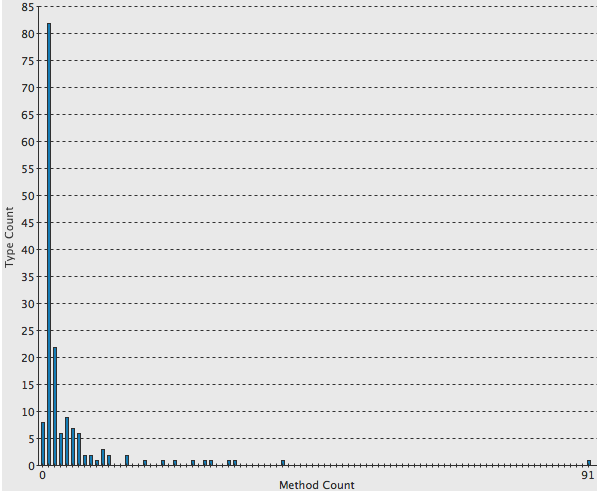
\includegraphics[height=10cm]{img/PQ/NumberOfMethodsPerType.png}
\caption{Sistema generale - Numero di metodi per tipo}
\end{figure}

\begin{figure}[htbp]
  \centering
  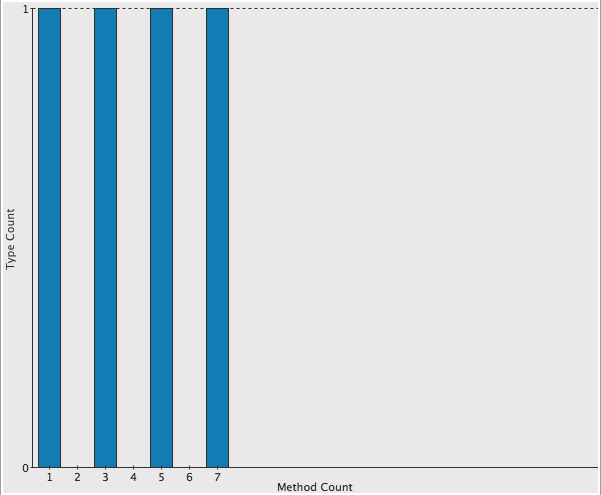
\includegraphics[height=10cm]{img/PQ/NumberOfMethodsPerTypeAPPLET.png}
\caption{Applet - Numero di metodi per tipo}
\end{figure}

\begin{figure}[htbp]
  \centering
  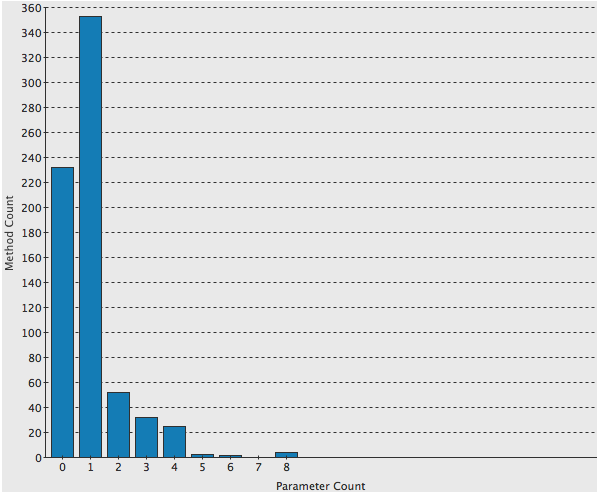
\includegraphics[height=10cm]{img/PQ/NumberOfParameters.png}
\caption{Sistema generale - Numero di parametri per metodo}
\end{figure}

\begin{figure}[htbp]
  \centering
  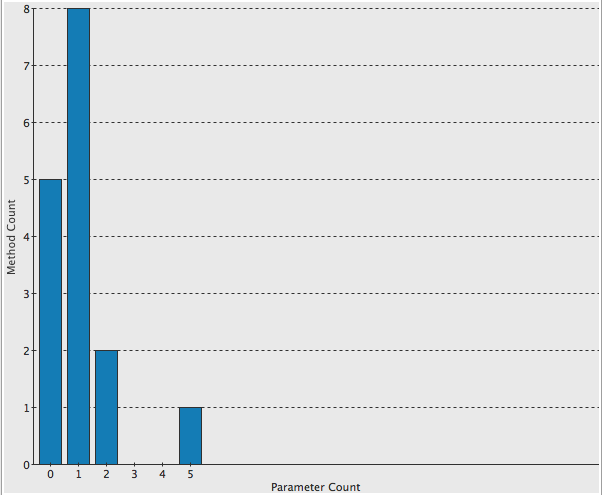
\includegraphics[height=10cm]{img/PQ/NumberOfParametersAPPLET.png}
\caption{Applet - Numero di parametri per metodo}
\end{figure}

\newpage

Le violazioni rispetto ai valori di soglia impostati sono:

\begin{itemize}
     \item \bo{Sistema generale:}
  \begin{itemize}
  \item Number of Types: it.unipd.netmus.client.ui con valore=\bo{99};
  \item Number of Methods Per Type: AppletConstants.java con valore=\bo{16.00};
  \item Number of Methods Per Type: MyConstants.java con valore=\bo{22.00};
  \item Number of Methods Per Type: Song.java con valore=\bo{37.00};
  \item Number of Methods Per Type: UserAccount.java con valore=\bo{34.00};
  \item Number of Methods Per Type: SongDTO.java con valore=\bo{18.00};
  \item Number of Methods Per Type: UserDTO.java con valore=\bo{20.00};
  \item Lines of Code: ProfileViewImpl.java con valore=\bo{2.169};
  \item Block Depth: LoginGoogleCallbackServlet.java con valore=\bo{5.00};
  \item Cyclomatic Complexity: BCrypt.java con valore=\bo{4.14}.
  \end{itemize}
    \item \bo{Applet}:
  \begin{itemize}
  \item Cyclomatic Complexity: DeviceScanner.java con valore=\bo{4.12};
  \item Cyclomatic Complexity: TranslateXML.java con valore=\bo{30.00}.
  \end{itemize}
\end{itemize}
Tutte queste violazioni sono state controllate e il sovraccarico rispetto ai
valori di soglia \`e dovuto al fatto che per motivi funzionali e
implementativi sono state progettate in questa maniera. 
\\\\
Il package
\emph{client.ui} \`e il package che contiene l'implementazione della GUI ed
essendo la grafica la parte pi\`u pesante del sistema, \`e normale che ci
sia questa abbondanza di classi ed \`e giustificata la violazione. \emph{AppletConstants.java} e \emph{MyConstants.java} hanno dei metodi che
restituiscono varie stringhe in lingue diverse e le violazioni rispetto l'alto numero di
metodi sono giustificate. \emph{Song.java} \`e una classe molto complessa e
dovendo mantenere molti campi dati e metodi per ogni canzone, \`e giustificata
la sua violazione. \emph{UserAccount.java} contiene tutte le
informazioni dell'account di ogni utente ed \`e corretto che contenga un numero
di metodi che supera la soglia prestabilita. \emph{SongDTO.java} e
\emph{UserDTO.java} contengono tutti i setter e getter delle classi
\emph{Song.java} e \emph{UserAccount.java} che hanno molti campi dati, e sono
giustificate le loro violazioni. \emph{ProfileViewImpl.java} \`e la classe che
gestisce tutta la view principale del sistema ed \`e corretto che sia cos\`i
complessa. \emph{LoginGoogleCallbackServlet.java} deve autenticare un utente con
account Google ed \`e corretto che abbia questo livello di annidamento.
\emph{BCrypt.java} serve per fare la cifratura della password, il suo livello di
complessit\`a ciclomatica \`e appena sopra la soglia ed \`e giustificata.
\emph{DeviceScanner.java} utilizza un algoritmo ricorsivo per fare ricerca di
file mp3 all'interno della cartella scelta ed \`e normale che abbia un
alto livello di complessit\`a ciclomatica. \emph{TranslateXML.java}
recupera le informazioni dai tag di un file mp3 e le inserisce in un file XML,
\`e corretto che abbia un alto livello di complessit\`a ciclomatica.

\section{Dettaglio delle verifiche tramite prove (test)}
Qui di seguito illustriamo i risultati dei test precedentemente trattati.
\subsection{Test di Unit\`a}

\begin{footnotesize}
\centering
\begin{longtable}{|p{5.7cm}|p{10.3cm}|}
\hline
\rowcolor{orange} \bo{Test di Unit\`a}  & \bo{Esiti} \\
\hline
\endhead
\hline
\multicolumn{2}{|c|}{\textit{continua alla pagina successiva}}\\
\hline
\endfoot
\endlastfoot
    
  \bo{TU-Cclac2}: ProfileActivity. &
  \textbf{Metodo}: setPlaylistList/getPlaylistList.\\&
  \textbf{Esito}: i metodi funzionano correttamente secondo la
  strategia adottata e soddisfano le aspettative programmate.\\&
  \textbf{Malfunzionamenti rilevati}: nessuno.\\&
  \\&
  \textbf{Metodo}: setFriendList/getFriendList.\\&
  \textbf{Esito}: i metodi funzionano correttamente secondo la
  strategia adottata e soddisfano le aspettative programmate.\\&
  \textbf{Malfunzionamenti rilevati}: nessuno.\\&
  \\&
  \textbf{Metodo}: rateSong.\\&
  \textbf{Esito}: il metodo funziona correttamente secondo la strategia
  adottata e soddisfa le aspettative programmate.\\& 
  \textbf{Malfunzionamenti
  rilevati}: nessuno.\\&
  \\&
  \textbf{Metodo}: playYouTube (1).\\&
  \textbf{Esito}: il metodo funziona correttamente secondo la strategia
  adottata e soddisfa le aspettative programmate.\\&
  \textbf{Malfunzionamenti rilevati}: nessuno.\\&
  \\&
  \textbf{Metodo}: playYouTube (2).\\&
  \textbf{Esito}: il metodo funziona correttamente secondo la strategia
  adottata e soddisfa le aspettative programmate.\\&
  \textbf{Malfunzionamenti rilevati}: nessuno.\\&
  \\&
  \textbf{Metodo}: setSongs/getSongs.\\&
  \textbf{Esito}: i metodi funzionano correttamente secondo la
  strategia adottata e soddisfano le aspettative programmate.\\&
  \textbf{Malfunzionamenti rilevati}: nessuno.\\&
  \\&
  \textbf{Metodo}: removeFromPlaylist (1).\\&
  \textbf{Esito}: il metodo funziona correttamente secondo la strategia
  adottata e rispecchia le aspettative programmate.\\&
  \textbf{Malfunzionamenti rilevati}: nessuno.\\&
  \\&
  \textbf{Metodo}: removeFromPlaylist (2).\\&
  \textbf{Esito}: il metodo funziona correttamente secondo la strategia
  adottata e soddisfa le aspettative programmate.\\&
  \textbf{Malfunzionamenti rilevati}: non viene gestito l'errore di rimozione,
  ma semplicemente il metodo chiama ``onFailure" che non fa nulla.\\&
  \\&
  \textbf{Metodo}: deletePlaylist (1).\\&
  \textbf{Esito}: il metodo funziona correttamente secondo la strategia
  adottata e soddisfa le aspettative programmate.\\&
  \textbf{Malfunzionamenti rilevati}: nessuno.\\&
  \\&
  \textbf{Metodo}: deletePlaylist (2).\\&
  \textbf{Esito}: il metodo funziona correttamente secondo la strategia
  adottata e soddisfa le aspettative programmate.\\&
  \textbf{Malfunzionamenti rilevati}: nessuno.\\&
  \\&
  \textbf{Metodo}: editProfile.\\&
  \textbf{Esito}: il metodo funziona correttamente secondo la strategia
  adottata e soddisfa le aspettative programmate.\\&
  \textbf{Malfunzionamenti rilevati}: nessuno.\\&
  \\&
  \textbf{Metodo}: setSongCover.\\&
  \textbf{Esito}: il metodo funziona correttamente secondo la strategia
  adottata e soddisfa le aspettative programmate.\\&
  \textbf{Malfunzionamenti rilevati}: nessuno.\\&
  \\&
  \textbf{Metodo}: calculatePreferredArtist.\\&
  \textbf{Esito}: il metodo funziona correttamente secondo la strategia
  adottata e soddisfa le aspettative programmate.\\&
  \textbf{Malfunzionamenti rilevati}: nessuno.\\&
  \\&
  \textbf{Metodo}: calculateSongStatistics.\\&
  \textbf{Esito}: il metodo funziona correttamente secondo la strategia
  adottata e soddisfa le aspettative programmate.\\&
  \textbf{Malfunzionamenti rilevati}: nessuno.\\&
  \\
  
  \hline
  \bo{TU-Cclac1}: LoginActivity. &
  \textbf{Metodo}: sendLogin (1).\\&
  \textbf{Esito}: il metodo funziona correttamente secondo la strategia
  adottata e soddisfa le aspettative programmate.\\&
  \textbf{Malfunzionamenti rilevati}: nessuno.\\&
  \\&
  \textbf{Metodo}: sendLogin (2).\\&
  \textbf{Esito}: il metodo funziona correttamente secondo la strategia
  adottata e soddisfa le aspettative programmate.\\&
  \textbf{Malfunzionamenti rilevati}: nessuno.\\&
  \\
  
  \hline
  \bo{TU-Cclap3}: TranslateDTOXML. &
  \textbf{Metodo}: XMLToDTO.\\&
  \textbf{Esito}: il metodo funziona correttamente, ma all'immissione
  di caratteri speciali diversi dalla codifica ISO-8859-1 il brano non viene
  impostato in un DTO ma viene direttamente saltato, passando alla creazione
  del DTO successivo.\\&
  \textbf{Malfunzionamenti rilevati}: non traduce in DTO i
  dati di una canzone che hanno una codifica diversa dalla ISO-8859-1, come ad
  esempio i caratteri giapponesi.\\& 
  \\

  \hline 
  \bo{TU-Cse5}: UserServiceImpl. &
  \textbf{Metodo}: editProfile.\\&
  \textbf{Esito}: il metodo funziona correttamente secondo la strategia
  adottata e soddisfa le aspettative programmate.\\& 
  \textbf{Malfunzionamenti rilevati}: nessuno.\\&
  \\
  
  \hline
  \bo{TU-Cse3}: SongServiceImpl. &
  \textbf{Metodo}: deleteSong.\\&
  \textbf{Esito}: il metodo funziona correttamente secondo la strategia
  adottata e soddisfa le aspettative programmate.\\& 
  \textbf{Malfunzionamenti rilevati}: nessuno.\\&
  \\
  
  \hline
  \bo{TU-Cse4}: LoginServiceImpl. &
  \textbf{Metodo}: restartSession.\\&
  \textbf{Esito}: il metodo funziona correttamente secondo la strategia
  adottata e soddisfa le aspettative programmate.\\&
  \textbf{Malfunzionamenti rilevati}: nessuno.\\&
  \\
  
  \hline
  \bo{TU-Cse6}: LibraryServiceImpl. &
  \textbf{Metodo}: sendUserNewMusic (1).\\&
  \textbf{Esito}: il metodo funziona correttamente secondo la strategia
  adottata e soddisfa le aspettative programmate.\\&
  \textbf{Malfunzionamenti rilevati}: nessuno.\\&
  \\&
  \textbf{Metodo}: sendNewUserMusic (2).\\&
  \textbf{Esito}: il metodo funziona correttamente secondo la strategia
  adottata e soddisfa le aspettative programmate.\\&
  \textbf{Malfunzionamenti rilevati}: il metodo non fa nulla in caso di errore,
  non resituisce alcun dato.\\&
  \\&
  \textbf{Metodo}: generatePdf.\\&
  \textbf{Esito}: il metodo funziona correttamente secondo la strategia
  adottata e soddisfa le aspettative programmate.\\&
  \textbf{Malfunzionamenti rilevati}: nessuno.\\&
  \\
  
  \hline
  \bo{TU-Csepe5}: UserAccount. &
  \textbf{Metodo}: findSessionUser.\\&
  \textbf{Esito}: il metodo funziona correttamente secondo la strategia
  adottata e soddisfa le aspettative programmate.\\&
  \textbf{Malfunzionamenti rilevati}: nessuno.\\&
  \\&
  \textbf{Metodo}: deleteUser.\\&
  \textbf{Esito}: il metodo funziona correttamente secondo la strategia
  adottata e soddisfa le aspettative programmate.\\&
  \textbf{Malfunzionamenti rilevati}: nessuno.\\&
  \\
  
  \hline
  \bo{TU-Csepe2}: MusicLibrary. &
  \textbf{Metodo}: removeSong.\\&
  \textbf{Esito}: il metodo funziona correttamente secondo la strategia
  adottata e soddisfa le aspettative programmate.\\&
  \textbf{Malfunzionamenti rilevati}: nessuno.\\&
  \\&
  \textbf{Metodo}: addSong.\\&
  \textbf{Esito}: il metodo funziona correttamente secondo la strategia
  adottata e soddisfa le aspettative programmate.\\&
  \textbf{Malfunzionamenti rilevati}: nessuno.\\&
  \\&
  \textbf{Metodo}: moveSong.\\&
  \textbf{Esito}: il metodo funziona correttamente secondo la
  strategia adottata e soddisfa le aspettative programmate.\\&
  \textbf{Malfunzionamenti rilevati}: nessuno.\\&
  \\
 
 \hline
 \bo{TU-Csepe1}: Album. &
 \textbf{Metodo}: loadAlbum.\\&
 \textbf{Esito}: il metodo funziona correttamente secondo la strategia
  adottata e soddisfa le aspettative programmate.\\&
 \textbf{Malfunzionamenti rilevati}: nessuno.\\&
 \\&
 \textbf{Metodo}: getAlbumCoverLastFM.\\&
 \textbf{Esito}: il metodo funziona correttamente secondo la strategia
  adottata e soddisfa le aspettative programmate.\\&
 \textbf{Malfunzionamenti rilevati}: nessuno.\\&
 \\
 
 \hline
 \bo{TU-Csepe4}: Song. &
 \textbf{Metodo}: incompleteSong.\\&
 \textbf{Esito}: il metodo funziona correttamente secondo la strategia
  adottata e soddisfa le aspettative programmate.\\&
 \textbf{Malfunzionamenti rilevati}: nessuno.\\&
 \\
 
\hline
\caption{Esiti dei Test di Unit\`a}
\end{longtable}
\end{footnotesize} 


Come si pu\`o chiaramente notare dagli esiti dei test sopra elencati, le prove
finora programmate e verificate hanno avuto tutti esiti positivi. Solo nei primi
test erano stati rilevati dei problemi di codifica, che sono stati
successivamente risolti.
  
\subsection{Test di Integrazione}

\begin{footnotesize}
\centering
\begin{longtable}{|p{5.7cm}|p{10.3cm}|}
\hline
\rowcolor{orange} \bo{Test di Integrazione}  & \bo{Esiti} \\
\hline
\endhead
\hline
\multicolumn{2}{|c|}{\textit{continua alla pagina successiva}}\\
\hline
\endfoot
\endlastfoot

  \bo{TI-se1} &
  \textbf{Esito}: le classi funzionano correttamente secondo la
  strategia adottata e soddisfano le aspettative programmate.\\&
  \textbf{Malfunzionamenti rilevati}: nessuno.\\&
  \\
  
  \hline
  \bo{TI-se2} &
  \textbf{Esito}: le classi funzionano correttamente secondo la
  strategia adottata e soddisfano le aspettative programmate.\\&
  \textbf{Malfunzionamenti rilevati}: nessuno.\\&
  \\
  
  \hline
  \bo{TI-cl1} &
  \textbf{Esito}: le classi funzionano correttamente secondo la
  strategia adottata e soddisfano le aspettative programmate.\\&
  \textbf{Malfunzionamenti rilevati}: nessuno.\\&
  \\
  
  \hline
  \bo{TI-cl2} &
  \textbf{Esito}: le classi funzionano correttamente secondo la
  strategia adottata e soddisfano le aspettative programmate.\\&
  \textbf{Malfunzionamenti rilevati}: nessuno.\\&
  \\
  
  \hline
  \bo{TI-gl1} &
  \textbf{Esito}: le classi funzionano correttamente secondo la
  strategia adottata e soddisfano le aspettative programmate.\\&
  \textbf{Malfunzionamenti rilevati}: nessuno.\\&
  \\
  
  \hline
  \bo{TI-gl2} &
  \textbf{Esito}: le classi funzionano correttamente secondo la
  strategia adottata e soddisfano le aspettative programmate.\\&
  \textbf{Malfunzionamenti rilevati}: nessuno.\\&
  \\

\hline
\caption{Esiti dei Test di Integrazione}
\end{longtable}
\end{footnotesize}

Come si pu\`o notare, tutti i test di integrazione effettuati hanno avuto esiti
positivi. Inizialmente due di questi, TI-cl2 e TI-gl1, avevano evidenziato un
problema di codifica perch\'e la classe \co{TranslateDTOXML} non inseriva
caratteri con codifica diversa da ISO-8859-1, ma successivamente \`e stato
corretto.

\subsection{Test di Sistema}
\begin{footnotesize}
\begin{longtable}{|p{2,4cm}|p{2,4cm}|}
\hline
\rowcolor{orange} \bo{Requisito}  & \bo{Presenza} \\
\hline
\endhead
\hline
\multicolumn{2}{|c|}{\textit{continua alla pagina successiva}}\\
\hline
\endfoot
\endlastfoot
 
 C1FN-1 &X \\ \hline
 C1FN-1.1 &X  \\ \hline
 C1FN-1.1.1 &X  \\ \hline
 C1FN-1.1.2  &X  \\ \hline
 C1FN-1.1.3 &X  \\ \hline
 C1FD-1.1.4  &X  \\ \hline
 C1FN-1.2 &X  \\ \hline
 C1FN-1.2.1 &X  \\ \hline
 C1FN-1.3 &X  \\ \hline
 C1FN-1.3.1  &X  \\ \hline
 C1FD-1.3.2 &X  \\ \hline
 C1FO-1.3.3 &X  \\ \hline
 C1F0-1.3.4 &X  \\ \hline
 C1FN-1.4 &X  \\ \hline
 C1FN-1.4.1 &X  \\ \hline
 C1FN-1.4.2 &X  \\ \hline
 C1FN-1.4.3 &X  \\ \hline
 C1FD-1.4.4 &X  \\ \hline
 C1FD-1.5 &X  \\ \hline
 C1FD-1.7 &X  \\ \hline
 C1FD-1.7.1  &X  \\ \hline
 C1F0-1.7.2 &X  \\ \hline
 C1FD-1.8 &X  \\ \hline
 C1F0-1.8.1 &X  \\ \hline
 C1FN-1.9 &X  \\ \hline
 C1FN-1.9.1  &X  \\ \hline
 C1FN-1.9.2 &X  \\ \hline
 C1FN-1.9.5 &X  \\ \hline
 C1FO-1.9.3 &X  \\ \hline
 C1FD-1.10 &X  \\ \hline
 C1FN-1.13 &-  \\ \hline
 C1QD-1.5.1 &X  \\ \hline
 C1QN-1.9.4 &X  \\ \hline
 C1QN-1.9.6 &-  \\ \hline
 C1QN-1.6 &- \\ \hline
 C1QD-1.6.1&- \\ \hline
 C1QN-1.6.2&-   \\ \hline
 C1QN-2&X \\ \hline
 C1QO-2.1&X \\ \hline
 C1QN-2.3&-  \\ \hline
 C1QD-2.4&X  \\ \hline
 C1QN-2.6&-  \\ \hline
 C1QN-2.7&X    \\ \hline
 C1QN-3.1&-   \\ \hline
 C1QD-3.1.1&-    \\ \hline
 C1VN-1.12&- \\ \hline
 C1VN-1.13.1&-  \\ \hline
 C1VN-1.11&-  \\ \hline
 C1VD-1.5.2&X \\ \hline
 C1VD-1.5.3&-   \\ \hline
 C1VN-2.2&- \\ \hline
 C1VN-2.5&-  \\ \hline
 C2FN-1&X    \\ \hline
 C2FN-1.1&X    \\ \hline
 C2FN-1.2&X   \\ \hline
 C2FO-1.3&X    \\ \hline
 C2FD-1.4&X   \\ \hline
 C2FN-1.5&X   \\ \hline
 C2FO-1.6&X   \\ \hline
 C2FD-2&X    \\ \hline
 C2FN-3&X   \\ \hline
 C2FN-3.1&X   \\ \hline
 C2QD-1.7&X   \\ \hline
 C2QN-3.2&X   \\ \hline
 C2QN-4 &X  \\ \hline
 C2QD-4.1&-    \\ \hline
 C2QD-4.2&-   \\ \hline
 C2QD-4.3&X   \\ \hline
 C2QN-4.4&-  \\ \hline
 C2VD-4.5&-   \\ \hline
 C2VN-4.6&-    \\ \hline
 C2VN-4.7&-  \\ \hline

\caption{Check sulla presenza ed implementazione dei requisiti software nel
sistema completo}
\end{longtable}
\end{footnotesize}

\section{Dettaglio dell'esito delle revisioni}
Dopo ogni revisione che il gruppo affronta consegnando la documentazione
richiesta e presentando il lavoro svolto, il committente fornisce una
valutazione che \`e la media ponderata del voto sui documenti *0.67 e la
presentazione orale *0.33. Inoltre viene data una descrizione accurata
sulle sezioni critiche dei documenti, che il gruppo si impegna subito
nel correggere/modificare per poter proseguire nello sviluppo del prodotto con delle
basi verificate e corrette.

\subsubsection*{RR}
Il lavoro svolto e il materiale consegnato sono stati valutati modestamente. \`E
emerso che due documenti sono da correggere e rivedere completamente, nello
specifico il Piano di Progetto e il Piano di Qualifica, mentre gli altri documenti nel complesso
vanno abbastanza bene. \\ \\
In dettaglio, per soddisfare le richieste del committente sono state apportate
le seguenti modifiche:
\begin{itemize}
  \item generali: messo in forma tabulare il registro delle modifiche, corretti
  i riferimenti normativi e informativi;
  \item Norme di Progetto: aggiunte le norme riguardanti le varie fasi di
  progetto (pianificazione, analisi, progettazione e codifica) e i corrispondenti strumenti;
  \item Analisi dei Requisiti: riscritti tutti gli Use-Case, sistemate pre-condizioni e scenari,
  inserite delle descrizioni pi\`u dettagliate nelle figure;
  \item Piano di Progetto: riscritta tutta la pianificazione, corretta l'analisi
  dei rischi;
  \item Piano di Qualifica: aggiunte le tecniche, le metriche e le procedure per
  fare verifica in tutte le varie fasi di progetto, sistemata la verifica della
  documentazione, corretti i concetti di anomalia e discrepanza, aggiunto
  il resoconto delle attivit\`a di verifica;
  \item Glossario: corretto il termine LateX.
\end{itemize}

\subsubsection*{RP}
Il giudizio complessivo sui documenti consegnati e la presentazione \`e stato
buono. Tutti i documenti sono in generale sufficienti.  \\ \\ In dettaglio, per
soddisfare le richieste del committente sono state apportate le seguenti modifiche:
\begin{itemize}
  \item generali: il sommario \`e stato posizionato dopo la prima pagina del
  documento e in tutti i documenti sono state messe al singolare le parole
  inglesi usate in un contesto italiano;
  \item Norme di Progetto: aggiunti aspetti di metodo, strategia e procedura di
  lavoro per le attivit\`a di analisi e progettazione;
  \item Analisi dei Requisiti: aggiunte pre-/post-condizioni pi\`u dettagliate
  in UC1, corretto titolo di UC2, sistemate pre-condizioni e aggiunta una forma
  di privacy in UC1.1, argomentata maggiormente UC2.2;
  \item Specifica Tecnica: sistemate tutte le descrizioni delle
  tecnologie e dei design pattern, rifatte le fig. 2.6, 2.7, 2.8, 2.10 e
  aggiunte le relative legende e descrizioni esaustive, rifatti i diagrammi di
  sequenza e aggiunte le relative descrizioni, sistemata la descrizione
  della funzione profilePlace presente nella fig. 2.9, corretto il diagramma
  delle attivit\`a fig. 3.3, aggiunta giustificazione esplicita dei requisiti
  non tracciabili nella sezione 4.2.1;
  \item Piano di Progetto: sistemata la terminologia in base alla nomenclatura
  ISO/IEC 12207, inserita una riga di totale in tutte le tabelle e rivisitato il
  preventivo della fase RP-RQ per rientrare nel range del preventivo presentato in precedenza;
  \item Piano di Qualifica: il capitolo sul ``Resoconto delle attivit\`a di
  verifica'' \`e stato messo in appendice, sistemate le sezioni 2.4 e 2.5;
  \item Glossario:  sistemati i caratteri con codifica non ASCII.
\end{itemize}

\subsubsection*{RQ}
Il giudizio complessivo sui documenti consegnati e la presentazione \`e stato
buono. Tutti i documenti sono in generale sufficienti.  \\ \\ In dettaglio, per
soddisfare le richieste del committente sono state apportate le seguenti modifiche:
\begin{itemize}
  \item Norme di Progetto: correzione di alcuni errori ortografici e
  sistemazione dello stile nelle titolazioni delle sezioni;
  \item Specifica Tecnica: argomentata la dipendenza tra \emph{server} e
  \emph{client.service}, ampliato le descrizioni dei diagrammi di sequenza e
  corretta la fig. 3.3;
  \item Definizione del Prodotto: correzione di alcuni errori
  ortografici e semantici, sistemato il sommario, aggiunti i documenti ST e AR
  come riferimenti informativi, aggiunte informazioni riportate in fig. 4.1 e
  4.2, tolte le relazioni con le altre componenti perch\'e gi\`a presenti nel
  documento ST, aggiunta la descrizione della fig. 4.2, sistemato
  ``testi\_vari'' in pag. 56, controllato la fig. 4.7 e deciso di
  lasciare invariata la componente \emph{server} perch\`e considerata gi\`a
  abbastanza riusabile, indicato il package della classe Exception
  in pag. 113, -------(VIEW GIOVI)-------;
  \item Manuale Utente: tolti i riferimenti a documento di
  progettazione/sviluppo, aggiunta descrizione per accedere al form di
  registrazione, aggiunta di un'individuazione grafica per le informazioni
  descritte nelle figure, sistemate le fig. 3.8 e 3.9, legate maggiormente fra
  loro le immagini e le descrizioni, completata l'ultima parte del documento,
  
  ----------DA FARE: Sez. 1.4: essendo la procedura di segnalazione di un errore
  descritta ``per passi'', converr\`a inserire screenshot / Sez. 3.2: ``della
  pi\`u interessante del nostro'' non \`e italiano / Rivedere il processo di
  rimozione di un brano, perch\'e troppo simile al processo di chiusura della
  finestra di dettaglio e quindi fonte di rischio.. ------------;
  \item Piano di Progetto: spostato l'intero cap. 5 in fondo al documento;
  \item Piano di Qualifica: correzione di alcuni errori ortografici, esiti delle
  verifiche tramite test messi in forma tabulare,
   -------(per ogni non
  conformit\`a rilevata fornire una giustificazione analitica e mettere i TU in
  appendice - ALBE)-------.
\end{itemize}

\subsubsection*{RA}
Per questa revisione non ci sar\`a esito prima del 21/03/2011.

\section{Dettaglio dell'esito nel test di valutazione sul\\ processo di lavoro}
I dati raccolti in questa fase di progetto rispetto agli ambiti ricoperti
(lavoro svolto, interazione con gli altri, strumenti utilizzati, tempo
impiegato), sono stati rappresentati in quattro grafici e riportati di seguito.
Nei grafici sono stati riportati in ascissa il ``Numero del Ticket'' (per avere
informazioni dettagliate sul ticket corrispondente riferirsi al link
\url{http://code.google.com/p/netmus/issues/list}) e in ordinata la
``Soddisfazione''.

\begin{figure}[htbp]
  \centering
  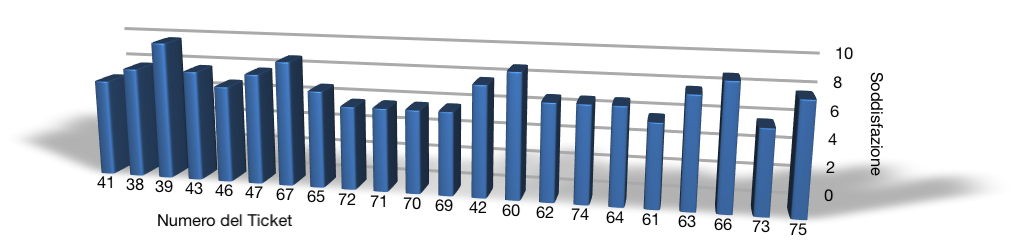
\includegraphics[height=4.1cm]{img/PQ/LavoroSvolto.png}
\caption{Feedback processo di lavoro - Lavoro svolto}
\end{figure}

\begin{figure}[htbp]
  \centering
  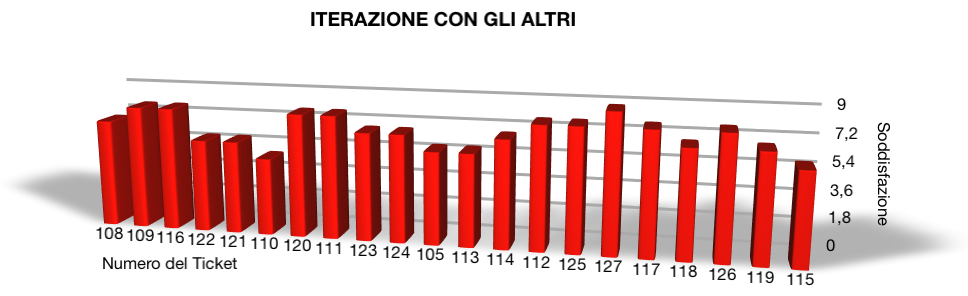
\includegraphics[height=4.1cm]{img/PQ/IterazioneConGliAltri.png}
\caption{Feedback processo di lavoro - Interazione con gli altri}
\end{figure}

\begin{figure}[htbp]
  \centering
  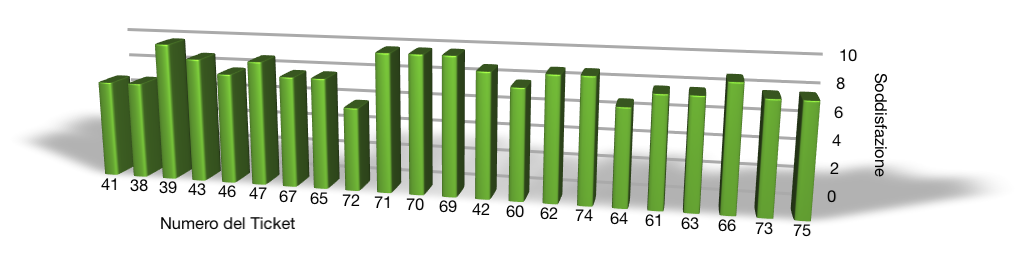
\includegraphics[height=4.1cm]{img/PQ/Strumenti.png}
\caption{Feedback processo di lavoro - Strumenti utilizzati}
\end{figure}

\begin{figure}[htbp]
  \centering
  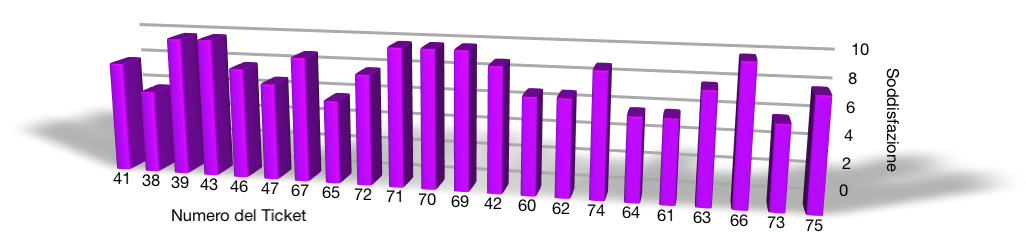
\includegraphics[height=4.1cm]{img/PQ/TempoImpiegato.png}
\caption{Feedback processo di lavoro - Tempo Impiegato}
\end{figure}

\newpage
I test di valutazione compilati in questa fase sono stati 21 e mostrano che
per:
\begin{itemize}
  \item il lavoro svolto, i membri del gruppo sono abbastanza
  soddisfatti (media voto 6.8);
  \item l'iterazione con gli altri, i membri del gruppo sono
  abbastanza soddisfatti (media voto 7.1);
  \item gli strumenti utilizzati, i membri del gruppo
  sono soddisfatti (media voto 7.5);
  \item il tempo impiegato, i membri del gruppo
  sono soddisfatti (media voto 7.4).\\
\end{itemize}

Questi risultati verranno confrontati con le valutazioni che si riceveranno
nella revisione RA e potranno fornire interessanti spunti su come correggere o
rafforzare il metodo di lavoro.

\subsubsection*{Conclusioni in relazione alle varie revisioni}

\begin{figure}[htbp]
  \centering
  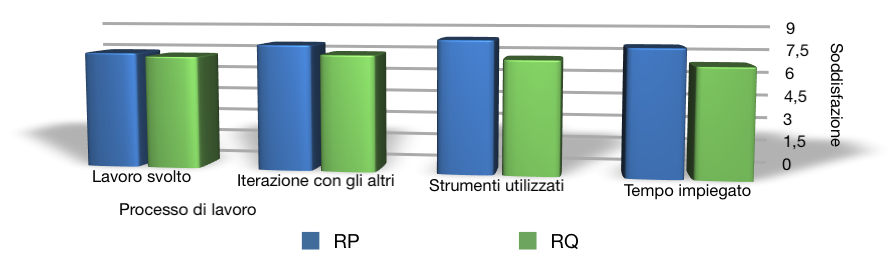
\includegraphics[height=4.5cm]{img/PQ/RiassuntoFeedback.png}
\caption{Medie dei feedback processo di lavoro per ogni revisione}
\end{figure}

Considerando l'esito della revisione RQ e le
valutazioni espresse nelle soddisfazioni dei processi di lavoro in quella
fase, si pu\`o dedurre che il gruppo ha lavorato bene, che \`e stato soddisfatto
del materiale prodotto e che la qualit\`a dei propri metodi di lavoro \`e stata
buona. \\ \\ 
Dalla figura A.5 si nota che il grado di soddisfazione generale tra la revisione
RP e la revisione RQ \`e calato di qualche punto e lo si pu\`o ricondurre al
fatto che in questa fase il gruppo si \`e fatto carico di un'ulteriore
revisione interna (``Progettazione nel dettaglio'') e il proprio livello di
stress \`e aumentato ulteriormente. Tra la revisione RQ e la revisione RA la
soddisfazione rispetto al lavoro svolto e all'iterazione con gli altri \`e
diminuita per motivi di stress dovuti alla lunga collaborazione e al
collaudo del prodotto imminente, mentre rispetto
all'utilizzo degli strumenti e al tempo impiegato \`e aumentata di qualche
punto.


\chapter{Tabella per la verifica dei documenti}
\thispagestyle{fancy}

\vspace{1cm}
\begin{table}[h]
\begin{center}
\begin{tabular}{|p{5cm}|p{4cm}|p{6cm}|}
\hline
\rowcolor{orange}
\bo{Tipo di errore}  & \bo{Posizione}  & \bo{Note e commenti} \\
\hline 
 &  & \\ \hline
 &  & \\ \hline
 &  & \\ \hline
 &  & \\ \hline
 &  & \\ \hline
 &  & \\ \hline
 &  & \\ \hline
 &  & \\ \hline
 &  & \\ \hline
 &  & \\ \hline
 &  & \\ \hline
 &  & \\ \hline
 &  & \\ \hline
 &  & \\ \hline
 &  & \\ \hline
 &  & \\ \hline


\end{tabular}
\caption{Tabella per la verifica dei documenti}
\end{center}
\end{table}

\subsubsection*{Tipi di errori:}

\begin{itemize}
\item Semantico grammaticale;
\item Chiarezza;
\item Concetto Generico;
\item Concetto Scorretto;
\item Concetto Incompleto.
\end{itemize}

\chapter{Tabella per il check dei requisiti}
\thispagestyle{fancy}

\vspace{1cm}
\begin{table}[h]
\begin{center}
\begin{tabular}{|p{2cm}|p{1,3cm}|p{1,3cm}|p{1,3cm}|p{1,3cm}|p{1,3cm}|p{1,3cm}|}
\hline
\rowcolor{orange}
\bo{Requisito}  & \bo{Corr.}  & \bo{Comp.}  & \bo{Ambi.}  & \bo{Veri.}  &
\bo{Cons.}  & \bo{Trac.} \\
\hline 
 &  &  &  &  &  & \\ \hline
 &  &  &  &  &  & \\ \hline
 &  &  &  &  &  & \\ \hline
 &  &  &  &  &  & \\ \hline
 &  &  &  &  &  & \\ \hline
 &  &  &  &  &  & \\ \hline
 &  &  &  &  &  & \\ \hline
 &  &  &  &  &  & \\ \hline
 &  &  &  &  &  & \\ \hline
 &  &  &  &  &  & \\ \hline
 &  &  &  &  &  & \\ \hline
 &  &  &  &  &  & \\ \hline
 &  &  &  &  &  & \\ \hline
 &  &  &  &  &  & \\ \hline
 &  &  &  &  &  & \\ \hline
 &  &  &  &  &  & \\ \hline
 &  &  &  &  &  & \\ \hline
 &  &  &  &  &  & \\ \hline
 &  &  &  &  &  & \\ \hline
 &  &  &  &  &  & \\ \hline
 &  &  &  &  &  & \\ \hline
 &  &  &  &  &  & \\ \hline
 &  &  &  &  &  & \\ \hline
 &  &  &  &  &  & \\ \hline
 &  &  &  &  &  & \\ \hline
 &  &  &  &  &  & \\ \hline
 &  &  &  &  &  & \\ \hline
 &  &  &  &  &  & \\ \hline
\end{tabular}
\caption{Tabella per il check dei requisiti}
\end{center}
\end{table}


\chapter{Tabella per il modello FURPS}
\thispagestyle{fancy}

\vspace{1cm}
\begin{table}[h]
\begin{center}
\begin{tabular}{|p{2cm}|p{1,3cm}|p{1,3cm}|p{1,3cm}|p{1,3cm}|p{1,3cm}|p{1,3cm}|}
\hline
\rowcolor{orange}
\bo{Requisito}  & \bo{F.}  & \bo{U.}  & \bo{R.}  & \bo{P.}  &
\bo{S.}\\
\hline 
 &  &  &  &  & \\ \hline
 &  &  &  &  & \\ \hline
 &  &  &  &  & \\ \hline
 &  &  &  &  & \\ \hline
 &  &  &  &  & \\ \hline
 &  &  &  &  & \\ \hline
 &  &  &  &  & \\ \hline
 &  &  &  &  & \\ \hline
 &  &  &  &  & \\ \hline
 &  &  &  &  & \\ \hline
 &  &  &  &  & \\ \hline
 &  &  &  &  & \\ \hline
 &  &  &  &  & \\ \hline
 &  &  &  &  & \\ \hline
 &  &  &  &  & \\ \hline
 &  &  &  &  & \\ \hline
 &  &  &  &  & \\ \hline
 &  &  &  &  & \\ \hline
 &  &  &  &  & \\ \hline
 &  &  &  &  & \\ \hline
 &  &  &  &  & \\ \hline
 &  &  &  &  & \\ \hline
 &  &  &  &  & \\ \hline
 &  &  &  &  & \\ \hline
 &  &  &  &  & \\ \hline
 &  &  &  &  & \\ \hline
 &  &  &  &  & \\ \hline
 TOTALE&  &  &  &  & \\ \hline

\end{tabular}
\caption{Tabella per il modello FURPS}
\end{center}
\end{table}


\chapter{Specifica dei Test di Unit\`a}
\thispagestyle{fancy}

\begin{footnotesize}
\centering
\begin{longtable}{|p{5.7cm}|p{10.3cm}|}
\hline
\rowcolor{orange} \bo{Test di Unit\`a}  & \bo{Specifiche} \\
\hline
\endhead
\hline
\multicolumn{2}{|c|}{\textit{continua alla pagina successiva}}\\
\hline
\endfoot
\endlastfoot

\bo{TU-Cclac2}:  ProfileActivity. &
\textbf{Metodo}: setPlaylistList/getPlaylistList.\\&
\textbf{Obiettivo}: verificare che avvenga con successo l'estrazione dal DB
delle playlist e che vengano correttamente inserite nella view.\\&
\textbf{Strategia}: al getter passare uno stub con una notevole quantit\`a di di stringhe di playlist,
 e vedere se poi il setter le riceve correttamente e le passa tutte alla view.\\&
\textbf{Tipologia}: whitebox.\\&
\textbf{Aspettative}: anche con una notevole quantit\`a di playlist,
l'estrazione e il passaggio dei dati alla view non dovrebbe dare errori.\\&
\\&
\textbf{Metodo}: setFriendList/getFriendList.\\&
\textbf{Obiettivo}: verificare la lettura dal DB della lista di amici di un
utente, e verificare la corretta importazione e visualizzazione sulla view.\\&
\textbf{Strategia}: nel DB locale viene inserita una lista di amici
fittizia, il metodo getter deve estrarla correttamente e il setter deve inviarla
correttamente alla view.\\&
\textbf{Tipologia}: blackbox.\\&
\textbf{Aspettative}: il getter deve restituire una lista di stringhe con i nomi
degli amici e il setter deve inviarla correttamente alla view per la visualizzazione.\\&
\\&
\textbf{Metodo}: rateSong.\\&
\textbf{Obiettivo}: verificare la registrazione di un voto per il
brano corretto e la sua visualizzazione sulla view.\\&
\textbf{Strategia}: verranno passati degli stub con artista, titolo e album di
un brano insieme ad un voto indicativo, e la ricerca del brano sar\`a
effettuata su un DB locale in cui il brano sar\`a presente.\\&
\textbf{Tipologia}: whitebox.\\&
\textbf{Aspettative}: il metodo dovr\`a trovare tale canzone, quindi inviare i
dati per la registrazione del voto sia al DB che alla view.\\&
\\&
\textbf{Metodo}: playYouTube (1).\\&
\textbf{Obiettivo}: verificare che il
programma sia in grado di ottenere e successivamente di impostare e visualizzare una canzone in streaming tramite
player di youtube.\\&
\textbf{Strategia}: verranno passati artista titolo e album al metodo, sul DB
locale sar\`a presente tale brano con l'indirizzo di youtube, il metodo
dovr\`a trovare tale brano e ritornare l'indirizzo da passare successivamente
alla view.\\&
\textbf{Tipologia}: whitebox.\\&
\textbf{Aspettative}: la ricerca deve ottenere il brano corretto
da youtube in base alla canzone selezionata e deve aggiornare la view con la
visualizzazione di tale canzone in ascolto .\\& 
\\&
\textbf{Metodo}: playYouTube (2).\\&
\textbf{Obiettivo}: verificare che un video gi\`a caricato venga
riprodotto senza dover nuovamente ricercare il suo codice su youtube.\\&
\textbf{Strategia}: verr\`a passato al metodo le stringhe del titolo, album e
artista di una canzone gi\`a presente nella Map delle canzoni gi\`a caricate.\\&
\textbf{Tipologia}: whitebox.\\&
\textbf{Aspettative}: il metodo deve saltare la ricerca del codice per il
video di youtube e analizzare le informazioni che il client possiede gi\`a nella
Map e di conseguenza caricare il video.\\&
\\&
\textbf{Metodo}: setSongs/getSongs.\\&
\textbf{Obiettivo}: verificare la corretta estrazione e visualizzazione del
catalogo brani, qualora un utente sia loggato.\\& 
\textbf{Strategia}: verr\`a passato al metodo getter un DTO con le informazioni
riguardanti la libreria di un utente, il metodo si occupa semplicemente di
smistare e riorganizzare le canzoni in una lista di stringhe che verr\`a
restituita con le info artista, titolo e album. Il setter invece utilizzer\`a
il getter per passare le info alla view.\\&
\textbf{Tipologia}: blackbox.\\&
\textbf{Aspettative}: deve
restituire una lista di stringhe contenenti artista, titolo ed album corretti di
ogni canzone della libreria dell'utente, e deve permettere il corretto invio per
la visualizzazione di tali informazioni sulla view.\\&
\\&
\textbf{Metodo}: removeFromPlaylist (1).\\&
\textbf{Obiettivo}: verificare la rimozione di un brano da una
playlist.\\& 
\textbf{Strategia}: verranno passate al metodo le stringhe con nome playlist,
e poi titolo artista e album del brano da rimuovere, la ricerca e rimozione
del brano dal DB locale dovrebbe avere successo e quindi richiamare la
rimozione anche dalla view.\\&
\textbf{Tipologia}: whitebox.\\&
\textbf{Aspettative}: il metodo richiama la
rimozione del brano dalla playlist dell'utente e una volta che la rimozione ha
avuto successo dalla parte del DB la rimuove anche dalla parte della dalla parte
della view.\\&
\\&
\textbf{Metodo}: removeFromPlaylist (2).\\&
\textbf{Obiettivo}: verificare che se un brano non sia presente nella
playlist, non venga eliminato.\\&
\textbf{Strategia}: vengono passati titolo, artista e album di una canzone non
presente nella playlist.\\&
\textbf{Tipologia}: whitebox.\\&
\textbf{Aspettative}: la ricerca sul DB deve ovviamente avere esito
negativo, il metodo quindi non deve avere successo ed eseguire dunque il
metodo ``onFailure" che gestisce il fallimento dell'operazione.\\&
\\&
\textbf{Metodo}: deletePlaylist (1).\\&
\textbf{Obiettivo}: verificare la rimozione completa di una
playlist.\\& 
\textbf{Strategia}: verr\`a passata al metodo una stringa contentente il nome
di una playlist creata.\\& 
\textbf{Tipologia}: blackbox.\\&
\textbf{Aspettative}: la playlist deve essere correttamente rimossa e non
pi\`u visualizzabile sulla view.\\&
\\&
\textbf{Metodo}: deletePlaylist (2).\\&
\textbf{Obiettivo}: verificare che il metodo qualora venga passata
una stringa con il nome di una playlist inesistente, non ne rimuova alcuna.\\&
\textbf{Strategia}: verr\`a passata al metodo una stringa contentente il nome di
una playlist che non \`e mai stata creata.\\& 
\textbf{Tipologia}: whitebox.\\&
\textbf{Aspettative}: il metodo non deve fare nulla, le playlist presenti
devono rimanere tali.\\&
\\&
\textbf{Metodo}: editProfile.\\&
\textbf{Obiettivo}: verificare il corretto invio dei dati inseriti
nella modifica del profilo di un utente.\\&
\textbf{Strategia}: verranno passate le stringhe contenenti i dati del profilo..\\&
\textbf{Tipologia}: whitebox.\\&
\textbf{Aspettative}: ogni informazione dovr\`a essere registrata con successo
in ogni campo dell'oggetto UserDTO.\\&
\\&
\textbf{Metodo}: setSongCover.\\&
\textbf{Obiettivo}: verificare che venga caricata la stringa con
l'indirizzo esatto della cover dell'album della canzone.\\&
\textbf{Strategia}: verranno passate le stringhe artista, titolo e album della
canzone, pi\`u un riferimento all'HTMLPanel su cui verr\`a visualizzata la
cover.\\&
\textbf{Tipologia}: whitebox.\\&
\textbf{Aspettative}: il metodo deve caricare l'indirizzo della cover
corretta, e memorizzarlo con successo per la canzone desiderata, oltre a
comunicare alla view il caricamento della cover a tale indirizzo.\\&
\\&
\textbf{Metodo}: calculatePreferredArtist.\\&
\textbf{Obiettivo}: verificare che il calcolo dell'artista preferito
venga eseguito in modo corretto e con successo.\\&
\textbf{Strategia}: verr\`a passata al metodo una MAP con tutte le canzoni
ascoltate, cos\`i da poter avere una traccia da cui partire per il calcolo
dell'artista preferito.\\&
\textbf{Tipologia}: blackbox.\\&
\textbf{Aspettative}: il metodo deve ritornare la stringa contentente il
nome dell'artista prediletto dall'utente.\\&
\\&
\textbf{Metodo}: calculateSongStatistics.\\&
\textbf{Obiettivo}: verificare che il calcolo della canzone pi\`u
popolare su netmus e della canzone pi\`u popolare per l'utente in questione
vada a buon fine.\\&
\textbf{Strategia}: verr\`a passata al metodo una MAP con
tutte le canzoni ascoltate, cos\`i da poter avere una traccia da cui partire per
il calcolo delle statistiche.\\&
\textbf{Tipologia}: blackbox.\\&
\textbf{Aspettative}: il metodo
deve ritornare una lista con le stringhe delle informazioni delle canzoni
pi\`u gettonate.\\&
\\

\hline
\bo{TU-Cclac1}: LoginActivity. &
\textbf{Metodo}: sendLogin (1).\\&
\textbf{Obiettivo}: verificare che il metodo per l'invio delle
informazioni del login funzioni correttamente in tutte le sue condizioni.\\&
\textbf{Strategia}: verr\`a passato user e password in stringhe al metodo, la
presenza di tale utente nel DB locale dovr\`a dare esito positivo di login..\\& 
\textbf{Tipologia}: whitebox.\\&
\textbf{Aspettative}: il
metodo deve creare un loginDTO con le informazioni inserite dall'utente, 
inviarlo al DB locale per verificare la validit\`a e in caso di successo aprire
la pagina di profileView.\\&
\\&
\textbf{Metodo}: sendLogin (2).\\&
\textbf{Obiettivo}: verificare che il metodo per l'invio delle
informazioni del login gestisca in modo adatto i casi di errore.\\&
\textbf{Strategia}: verranno passate delle stringhe con nome e password
inesistenti nel DB.\\&
\textbf{Tipologia}: blackbox.\\&
\textbf{Aspettative}: il metodo deve restituire un messaggio di errore di
utente non registrato al sistema.\\&
\\

\hline
\bo{TU-Cclap3}:  TranslateDTOXML. &
\textbf{Metodo}: XMLToDTO.\\&
\textbf{Obiettivo}: questo metodo riceve in input una stringa XML che
contiene le informazioni di ogni brano estratto da un dispositivo. Estrae i
dati di ogni brano e restituisce una lista di oggetti SongDTO da inviare
successivamente alla componente di persistenza. Il test Vuole verificare la corretta creazione della lista di SongDTO.\\& 
\textbf{Strategia}: verr\`a passata una stringa xml con una quantit\`a
notevole di brani e con caratteri diversi anche dalla codifica ISO-8859-1.\\&
\textbf{Tipologia}: blackbox.\\&
\textbf{Aspettative}: il metodo dovr\`a ritornare una lista
di DTO di tutti i brani rilevati senza saltarne alcuno e con tutte le informazioni memorizzate nel
rispettivo campo..\\&
\\

\hline
\bo{TU-Cse5}:  UserServiceImpl. &
\textbf{Metodo}: editProfile.\\&
\textbf{Obiettivo}: verificare che l'operazione di editing e
salvataggio delle informazioni di un profilo vada a buon fine.\\&
\textbf{Strategia}: verr\`a passato al metodo un nome utente presente nel DB
locale e un DTO con le informazioni riguardanti l'account utente.\\&
\textbf{Tipologia}: whitebox.\\&
\textbf{Aspettative}: il metodo registrer\`a tutti i nuovi campi editati e
ritorner\`a true qualora l'operazione vada a buon fine.\\&
\\

\hline
\bo{TU-Cse6}: LibraryServiceImpl. &
\textbf{Metodo}: sendUserNewMusic (1).\\&
\textbf{Obiettivo}: verificare l'invio e la memorizzazione di una lista di
brani nuovi rilevati dal dispositivo dell'utente.\\& 
\textbf{Strategia}: verr\`a passato al metodo il nome dell'utente e una lista
di SongDTO che dovranno essere registrate sulla libreria virtuale.\\&
\textbf{Tipologia}: whitebox.\\&
\textbf{Aspettative}: corretta memorizzazione all'interno del DB
locale dell'utente selezionato di tutti i nuovi brani rilevati.\\&
\\&
\textbf{Metodo}: sendUserNewMusic (2).\\&
\textbf{Obiettivo}: verificare che l'invio e la memorizzazione di
una nuova lista di canzoni non avvenga se l'utente non viene trovato.\\&
\textbf{Strategia}: verranno passati al metodo un user inseistente ed una lista
di oggetti SongDTO.\\&
\textbf{Tipologia}: blackbox.\\&
\textbf{Aspettative}: il metodo non deve memorizzare tali canzoni, ma
ritornare un errore.\\&
\\&
\textbf{Metodo}: generatePdf.\\&
\textbf{Obiettivo}: verificare la creazione del PDF della libreria
dell'utente.\\&
\textbf{Strategia}: viene passato all'utente il nome dell'utente di cui creare
il PDF della propria libreria.\\&
\textbf{Tipologia}: blackbox.\\&
\textbf{Aspettative}: il metodo deve ritornare l'id del doc PDF contenente
la sua libreria musicale.\\&
\\

\hline
\bo{TU-Cse3}: SongServiceImpl. &
\textbf{Metodo}: deleteSong.\\&
\textbf{Obiettivo}: verificare la rimozione della canzone
selezionata dalla libreria dell'utente.\\&
\textbf{Strategia}: verr\`a passato al metodo le chiavi di un brano, ossia
artista, titolo e album, oltre al nome dell'utente da cui rimuovere il brano.
L'utente e il brano sono entrambi presenti nel DB locale, perci\`o il metodo
non dovrebbe avere errori.\\&
\textbf{Tipologia}: whitebox.\\&
\textbf{Aspettative}: deve rimuovere con successo dal DB locale il brano, e
ritornare true che indica che l'operazione \`e andata a buon fine.\\&
\\

\hline
\bo{TU-Cse4}: LoginServiceImpl. &
\textbf{Metodo}: restartSession.\\&
\textbf{Obiettivo}: verificare il corretto funzionamento durante il
recupero di una sessione per un utente.\\&
\textbf{Strategia}: verr\`a passato al metodo stringhe con nome utente e id
di sessione estratti da un cookie presente. Il recupero della sessione
dovrebbe andare a buon fine..\\&
\textbf{Tipologia}: whitebox.\\&
\textbf{Aspettative}: il metodo deve controllare l'effettiva esistenza
dell'utente loggato nella sessione attuale, successivamente caricher\`a
l'userAccount di tale utente e confronter\`a l'id della sessione con quello
dell'ultima sessione attiva dell'utente, infine aggiorner\`a i dati della
sessione con quelli dell'utente che l'ha appena recuperata.\\&
\\

\hline
\bo{TU-Csepe5}: UserAccount. &
\textbf{Metodo}: findSessionUser.\\&
\textbf{Obiettivo}: verificare il successo nella ricerca dell'id
dell'ultima sessione dell'utente.\\&
\textbf{Strategia}: verr\`a passato al metodo
l'id della sessione.\\&
\textbf{Tipologia}: blackbox.\\&
\textbf{Aspettative}: il metodo compone una query per il DB locale in cui
ricerca l'id dell'ultima sessione di lavoro dell'utente.\\&
\\&
\textbf{Metodo}: deleteUser.\\&
\textbf{Obiettivo}: verificare l'effettiva e corretta cancellazione di un
account dal DB e quindi dal sistema NetMus.\\&
\textbf{Strategia}: verr\`a passato al metodo un oggetto UserAccount, che
fornir\`a le chiavi per la ricerca e la cancellazione dell'account utente.\\&
\textbf{Tipologia}: whitebox.\\&
\textbf{Aspettative}: l'account dell'utente deve venire eliminato dal DB cos\`i
come tutti i suoi dati e la sua libreria.\\&
\\

\hline
\bo{TU-Csepe2}: MusicLibrary. &
\textbf{Metodo}: removeSong.\\&
\textbf{Obiettivo}: verificare la corretta rimozione del riferimento ad una
canzone dalla libreria nel DB di un utente.\\&
\textbf{Strategia}: al metodo verranno passati un oggetto di tipo Song e un
booleano che indica l'aggiornamento delle statistiche utente una volta
completata la rimozione.\\&
\textbf{Tipologia}: blackbox.\\&
\textbf{Aspettative}: viene ritornato true qualora la
cancellazione sia andata a buon fine, e che nella libreria dell'utente il brano
sia stato effettivamente rimosso.\\&
\\&
\textbf{Metodo}: addSong.\\&
\textbf{Obiettivo}: verificare la corretta registrazione di una nuova
canzone sul DB.\\&
\textbf{Strategia}: viene passato un oggetto Song al metodo che si occupa di
registrarne i campi, e una variabile booleana update per l'aggiornamento delle
statistiche dell'utente.\\&
\textbf{Tipologia}: blackbox.\\&
\textbf{Aspettative}: il metodo deve ricercare nel DB
la presenza della canzone che si sta cercando di aggiungere. In caso di match positivo, la canzone non viene aggiunta perch\`e gi\`a presente, in caso negativo viene registrata e i
campi corretti relativi alle informazioni della libreria vengono aggiornati.\\&
\\&
\textbf{Metodo}: moveSong.\\&
\textbf{Obiettivo}: verificare lo spostamento di una canzone nella
lista della playlist venga eseguito in modo corretto.\\&
\textbf{Strategia}: verr\`a passato un intero che indica la posizione, e per
l'occasione superer\`a il range della lista.\\&
\textbf{Tipologia}: blackbox.\\&
\textbf{Aspettative}: il metodo deve ritornare false, poich\`e non \`e
possibile spostare una canzone in una posizione fuori dal limite della lista.\\&
\\

\hline
\bo{TU-Csepe1}: Album. &
\textbf{Metodo}: loadAlbum.\\&
\textbf{Obiettivo}: verificare la lettura dal DB locale di un Album
non presente nella cache e di una sua successiva registrazione nella cache.\\&
\textbf{Strategia}: verr\`a passato al metodo la stringa contenente l'id di un
album non presente nella cache ma presente nel DB.\\&
\textbf{Tipologia}: whitebox.\\&
\textbf{Aspettative}: il metodo deve ritornare l'album estratto dal DB
locale e allo stesso tempo deve aver registrato nella cache il caricamento di
tale album.\\&
\\&
\textbf{Metodo}: getAlbumCoverLastFM.\\&
\textbf{Obiettivo}: verificare la ricerca di una copertina nel DB o
tramite servizio esterno di LastFM vada a buon fine.\\&
\textbf{Strategia}:
al metodo vengono passate le stringhe del nome dell'album e dell'artista .\\&
\textbf{Tipologia}: whitebox.\\&
\textbf{Aspettative}: tali stringhe non troveranno alcun match sul DB
locale, perci\`o verr\`a richiamato il servizio esterno di LastFM per la
ricerca delle copertine.\\&
\\

\hline
\bo{TU-Csepe4}: Song. &
\textbf{Metodo}: incompleteSong.\\&
\textbf{Obiettivo}: verificare che il reperimento delle informazioni
per una canzone incompleta vada a buon fine.\\&
\textbf{Strategia}:
viene passato al metodo un SongDTO con le informazioni del brano che risultano
incomplete.\\&
\textbf{Tipologia}: whitebox.\\&
\textbf{Aspettative}: il metodo deve ricercare nel DB se tale brano \`e
gi\`a presente, in modo da completarne le informazioni, oppure cerca di
estrapolare le informazioni dal nome del file.\\& \\

\hline
\caption{Test di Unit\`a previsti e relative specifiche}
\end{longtable}
\end{footnotesize}



\chapter{Specifica dei Test di Integrazione}
\thispagestyle{fancy}

\begin{footnotesize}
\centering
\begin{longtable}{|p{5.7cm}|p{10.3cm}|}
\hline
\rowcolor{orange} \bo{Test di Integrazione}  & \bo{Specifiche} \\
\hline
\endhead
\hline
\multicolumn{2}{|c|}{\textit{continua alla pagina successiva}}\\
\hline
\endfoot
\endlastfoot

\bo{TI-se1}: server, server.persistent, shared. &
\textbf{Classi coinvolte}: UserServiceImpl, SongsServiceImpl,
LibraryServiceImpl, UserAccount, Song, MusicLibrary, DatastoreUtils,
MusicLibraryDTO, SongDTO, UserCompleteDTO.\\& 
\textbf{Obiettivo}: verificare l'integrazione tra le classi che
forniscono un servizio al client e quelle che si interfacciano al database,
controllando che i servizi vengano forniti correttamente.\\& 
\textbf{Strategia}: verranno dati in input le informazioni di un nuovo utente,
alcuni brani casuali, ed un paio di playlist .\\&
\textbf{Aspettative}: dalle chiamate ai servizi dovranno essere restituiti
tutti i dati corretti dell'utente, le informazioni dei brani e delle playlist,
equivalenti ai dati inseriti.\\&
\\

\hline
\bo{TI-se2}: server, server.persistent, server.youtube, server.utils,
server.utils.cache, server.utils.velocity, shared. &
\textbf{Classi coinvolte}: UserServiceImpl, SongsServiceImpl,
LibraryServiceImpl, UserAccount, Song, MusicLibrary, DatastoreUtils,
YouTubeManager, YouTubeMedia, YouTubeTester, YouTubeVideo, ExternalService,
ServletUtils, Utils, Cacheable, ChacheSupport,
VelocityEngineManager, VelocityResourceLoader, MusicLibraryDTO, SongDTO,
UserCompleteDTO.\\&
\textbf{Obiettivo}: verificare il funzionamento e
l'interfacciamento coi servizi esterni.\\&
\textbf{Strategia}: verranno dati in input ai servizi le informazioni di un
nuovo utente e alcuni brani predefiniti con informazioni incomplete, di cui
si \`e sicuri che i servizi esterni possano aggiungere informazioni.\\&
\textbf{Aspettative}: dalle chiamate ai servizi dovranno essere restituiti quei
brani con i dati completati, come immagine dell'album e link al video youtube.\\&
\\

\hline
\bo{TI-cl1}: client, client.activity, client.mvp, client.service, shared. & 
\textbf{Classi coinvolte}: ClientFactoryImpl, ProfileActivity,
NetmusActivityMapper, LibraryService, SongsService, UsersService,
MusicLibraryDTO, SongDTO, UserCompleteDTO.\\&
\textbf{Obiettivo}: verificare il corretto funzionamento della
parte logica del client: vengono simulate alcune operazioni effettuate
dall'utente, e osservate le reazioni.\\&
\textbf{Strategia}: seguendo l'inizializzazione normale, come dato
in ingresso iniziale avremo una MusicLibrary, e si controller\`a il corretto
inserimento dei dati nello stub della view. In seguito saranno simulate varie
azioni dell'utente e si controller\`a se le reazioni seguiranno quanto
previsto.\\&
\textbf{Aspettative}: ci dovranno essere richieste dei dettagli dei brani ai
servizi, e l'inserimento degli stessi nello stub della view.\\&
\\

\hline
\bo{TI-cl2}: client, client.activity, client.mvp, client.service,
client.applet, shared. &
\textbf{Classi coinvolte}: ClientFactoryImpl, ProfileActivity,
NetmusActivityMapper, LibraryService, SongsService, UsersService, AppletBar,
TranslateDTOXML, MusicLibraryDTO, SongDTO, UserCompleteDTO.\\& 
\textbf{Obiettivo}: verificare l'integrazione dell'applet.\\&
\textbf{Strategia}: verr\`a dato in input un documento XML contenente dei brani
dallo stub dell'applet.\\& 
\textbf{Aspettative}: ci si aspettano delle chiamate ai servizi per aggiungere
i brani al database.\\&
\\

\hline
\bo{TI-gl1}: client, client.activity, client.mvp, client.service, client.applet,
server, server.persistent, server.youtube, server.utils, server.utils.cache,
server.utils.velocity, shared. &
\textbf{Classi coinvolte}: ClientFactoryImpl, ProfileActivity, NetmusActivityMapper,
LibraryService, SongsService, UsersService, AppletBar,
TranslateDTOXML, UserServiceImpl, SongsServiceImpl,
LibraryServiceImpl, UserAccount, Song, MusicLibrary, DatastoreUtils,
YouTubeManager, YouTubeMedia, YouTubeTester, YouTubeVideo, ExternalService,
ServletUtils, Utils, Cacheable, ChacheSupport,
VelocityEngineManager, VelocityResourceLoader, MusicLibraryDTO, SongDTO, UserCompleteDTO.\\& 
\textbf{Obiettivo}: verificare l'integrazione della componente
server e quella client.\\&
\textbf{Strategia}: verr\`a dato in input un documento XML contenente dei brani
dallo stub dell'applet.\\&
\textbf{Aspettative}: nello stub della view dovr\`a essere inserita una nuova
lista di brani, comprendente quelli nuovi indicati nell'XML.\\& 
\\

\hline
\bo{TI-gl2}: client, client.activity, client.mvp, client.service, client.applet,
server, server.persistent, server.youtube, server.utils, server.utils.cache,
server.utils.velocity, shared. &
\textbf{Classi coinvolte}: ClientFactoryImpl, ProfileActivity, NetmusActivityMapper,
LibraryService, SongsService, UsersService, AppletBar,
TranslateDTOXML, UserServiceImpl, SongsServiceImpl,
LibraryServiceImpl, UserAccount, Song, MusicLibrary, DatastoreUtils,
YouTubeManager, YouTubeMedia, YouTubeTester, YouTubeVideo, ExternalService,
ServletUtils, Utils, Cacheable, ChacheSupport,
VelocityEngineManager, VelocityResourceLoader, MusicLibraryDTO, SongDTO, UserCompleteDTO.\\& 
\textbf{Obiettivo}: verificare la gestione dell'account utente.\\&
\textbf{Strategia}: verr\`a creato un nuovo profilo utente, e
successivamente modificate le informazioni di quel profilo.\\&
\textbf{Aspettative}: le nuove informazioni inserite dovranno essere
inserite nel database, e inserite correttamente nella view.\\&
\\

\hline
\caption{Test di Integrazione previsti e relative specifiche}
\end{longtable}
\end{footnotesize}


\end{document}

